% !Mode:: "TeX:UTF-8"
\thispagestyle{empty}
\chapter{3D LiDAR Localization and Mapping}
\thispagestyle{empty}

This chapter introduces the principles of mapping and localization using 3D LiDAR. Compared to 2D LiDAR, 3D LiDAR provides richer information, is less susceptible to occlusion, and can better reconstruct the three-dimensional structure of the environment. We can either directly register the 3D point clouds or extract geometric features before registration. Both approaches are widely used in autonomous driving applications. In this chapter, we will manually implement the core algorithms and assemble them into a LiDAR odometry system.

\includepdf{art/ch7.pdf}

\section{Working Principles of Multi-beam LiDAR}
\subsection{Mechanical LiDAR}
The ranging principle of multi-beam LiDAR is the same as that of single-beam LiDAR. They emit a laser pulse toward the target object, measure the time interval between the transmitted and returned pulses, and then calculate the distance by multiplying the time interval by the speed of light. If the laser penetrates the object during measurement, the receiver may capture multiple echoes. Most LiDAR systems compute the distances from multiple echoes and use the strongest return as the final measured distance. This ranging principle is called Time of Flight (ToF), which is the primary method for most LiDAR sensors and RGB-D cameras. ToF can be further divided into Direct ToF (DToF) and Indirect ToF (IToF), with IToF further categorized into Frequency-Modulated Continuous Wave (FMCW) and Amplitude-Modulated Continuous Wave (AMCW). Due to its lower power consumption and simpler implementation, most LiDARs and RGB-D cameras currently use DToF for ranging.

Compared to single-beam LiDAR, multi-beam LiDAR typically has multiple laser emitters. These are controlled by motors and rotate around an axis at a fixed frequency (e.g., 10 revolutions per second). The laser emitters are arranged at small angular offsets, allowing them to scan objects within a certain field of view when rotating. This rotating configuration is called a \textbf{spinning LiDAR} or mechanical LiDAR. Mechanical LiDARs usually have a 360-degree horizontal field of view, while the vertical field of view depends on the emitter arrangement, typically ranging from 30 to 45 degrees. The number of emitters is referred to as the \textbf{channel count}. Due to their symmetrical design, the channel count is usually a power of two, with common configurations including 4, 16, 32, 64, and 128 channels. The complexity and cost increase significantly with higher channel counts. Figure~\ref{fig:3d-lidars}~ shows several common 3D LiDARs and their single-frame scan data, demonstrating their significantly richer information compared to 2D LiDARs.

\begin{figure}[!htp]
	\centering
	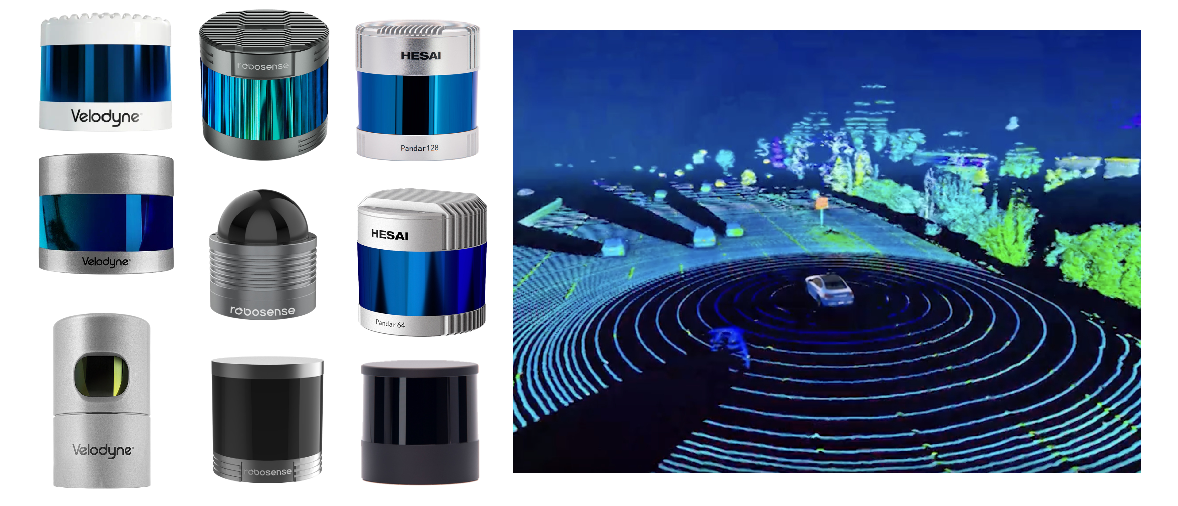
\includegraphics[width=0.8\textwidth]{resources/3d-lidar-mapping/3d-lidars.pdf}
	\caption{Common 3D LiDARs on the market and their single-frame scan data.}
	\label{fig:3d-lidars}
\end{figure}

The rich information provided by 3D LiDARs greatly simplifies many computational tasks. For example, we can detect vehicles, traffic signs, and other distinct objects in 3D point clouds \cite{Zhou2018,Shi2019}, identify static and dynamic obstacles, and extract lane markings using reflection intensity \cite{Sithole2003,Fernandes2021}—tasks that are challenging with 2D LiDAR. From a localization and mapping perspective, we can register multiple scans to create a global point cloud map. Annotators can then label the point cloud to generate a \textbf{high-definition (HD) map}, enabling vehicles to achieve \textbf{high-precision localization} within the map. This is currently the standard practice for many Level 4 (L4) autonomous vehicles.

\begin{figure}[!t]
	\centering
	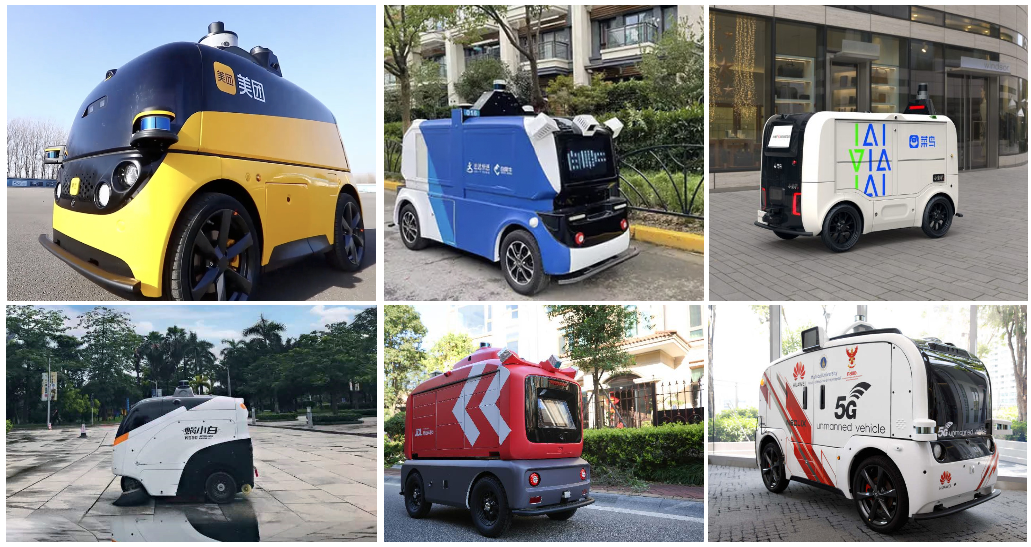
\includegraphics[width=0.8\textwidth]{resources/3d-lidar-mapping/low-speed-l4-cars.pdf}
	\caption{Low-speed autonomous vehicles using multi-beam LiDAR as the primary sensor}
	\label{fig:low-speed-l4-cars}
\end{figure}

In the early years, mechanical LiDARs were primarily supplied by Velodyne. However, with recent technological advancements, domestic manufacturers such as RoboSense, Hesai, and DJI have gradually taken over the market, while Velodyne has declined. Today, mechanical LiDARs are available at relatively reasonable prices, with cost-effective 16-channel LiDARs becoming the preferred choice for many low-speed autonomous driving products. Figure~\ref{fig:low-speed-l4-cars}~ shows some low-speed autonomous vehicles equipped with multi-beam LiDARs. These vehicles typically use one or more LiDARs for mapping and localization. To ensure unobstructed views, they commonly mount the LiDAR on the roof, allowing 360-degree coverage around the vehicle. However, due to the limited vertical field of view, roof-mounted LiDARs create significant blind spots near the vehicle. Some larger vehicles address this issue by installing one or two supplementary blind-spot LiDARs at the front to prevent collisions. Nevertheless, using multiple LiDARs significantly increases overall costs, posing a major challenge for mass production.

\subsection{Solid-State LiDAR}  
Mechanical LiDARs require rotating laser emitters to achieve 360-degree coverage, inevitably incorporating precision mechanical components. These moving parts lead to high costs and vulnerability under harsh conditions like vehicle vibrations. Consequently, LiDARs that measure distances without moving the entire emission/reception assembly—collectively termed \textbf{solid-state LiDARs} (see Fig.~\ref{fig:solid-lidars})—have emerged.  

Solid-state LiDARs employ various measurement principles:  
\begin{enumerate}  
	\item \textbf{Rotating Mirror (Semi-Solid) Design}: The laser emitter and receiver remain stationary, while a prism deflects the beam to scan different directions. Though the prism undergoes minor motion, this design eliminates rotating emitters. Examples include RoboSense and DJI's mass-produced rotating mirror LiDARs, now deployed in some passenger vehicles.  
	\item \textbf{Pure Solid-State Designs}:  
	\begin{itemize}  
		\item \textit{Phased Array}: Scans sequentially via electronic beam steering.  
		\item \textit{Flash LiDAR}: Illuminates the entire FoV simultaneously for single-shot 3D capture.  
	\end{itemize}  
	These technologies remain less mature but promise fully static operation.  
\end{enumerate}  

\begin{figure}[!t]  
	\centering  
	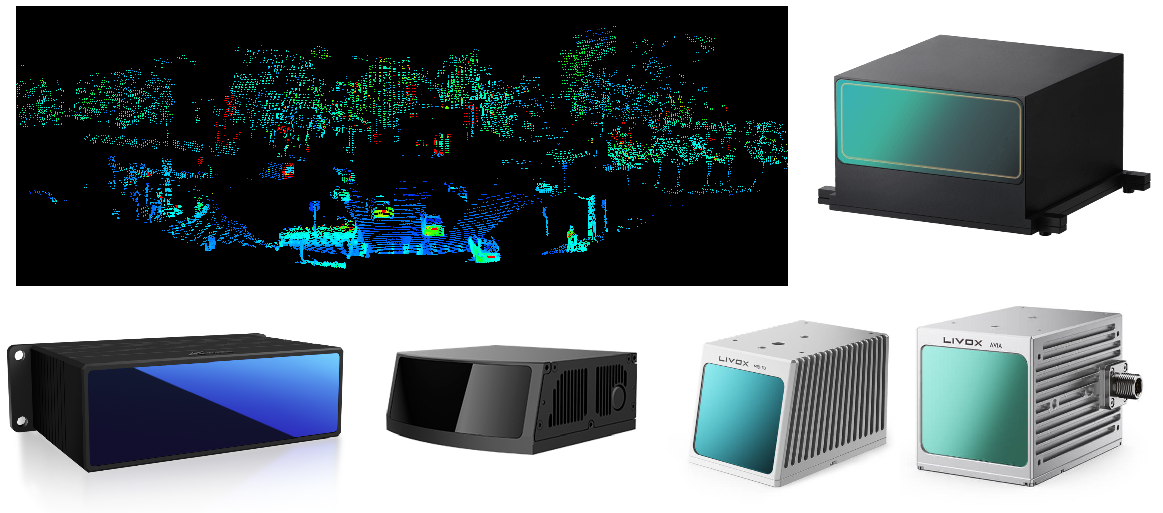
\includegraphics[width=0.8\textwidth]{resources/3d-lidar-mapping/solid-lidars.pdf}  
	\caption{Representative solid-state LiDARs and their scan patterns}  
	\label{fig:solid-lidars}  
\end{figure}  

Both semi- and pure solid-state LiDARs feature a scanning window defining their \textbf{Field of View (FoV)}. Typical horizontal FoVs are <120° (vs. 360° for mechanical LiDARs), while vertical FoVs are comparable. Unlike mechanical LiDARs, solid-state variants lack a \textbf{channel count} metric\footnote{Some manufacturers use "equivalent channels"; e.g., many solid-state LiDARs match 128-channel mechanical performance but with narrower FoVs.}. For instance, DJI's Livox series employs a "petal" scanning pattern, whereas others mimic mechanical LiDAR's horizontal scanning with equivalent channels. The constrained FoV enables higher scan rates at the cost of fewer points per frame. Ranging accuracy remains comparable as both types use ToF principles.  

With lower costs and extended lifespans, solid-state LiDARs are increasingly adopted in production vehicles—primarily for forward obstacle detection rather than L4 HD mapping/localization. While consumer vehicles may use 1–2 front-facing units, L4 systems often combine 4–5 solid-state LiDARs for 360° coverage, introducing calibration/synchronization challenges and eroding cost advantages over mechanical LiDARs.  

Most algorithms discussed later are agnostic to LiDAR type (mechanical/solid-state). We provide datasets for both to evaluate SLAM performance. Emerging designs (e.g., spherical/hemispherical FoV solid-state LiDARs) promise broader coverage, reflecting ongoing sensor evolution that will continue driving SLAM innovation.

\section{Scan Matching for Multi-beam LiDAR}  
The SLAM framework for multi-beam LiDAR is similar to that of single-beam systems. Following the previous chapter, we first discuss scan matching methods for aligning two point clouds, then address back-end processing. Multi-beam LiDAR typically yields superior scan matching compared to single-beam systems, simplifying back-end design. Most multi-beam SLAM systems forgo submap concepts, directly managing point clouds. Thus, registration primarily employs scan-to-scan or scan-to-map approaches.  

\subsection{Point-to-Point ICP}  
\subsubsection{Theoretical Foundations}  
Point-to-point Iterative Closest Point (ICP) is a fundamental point cloud registration method. Given two point clouds $S_1=\{\mathbf{p}_1, \ldots, \mathbf{p}_m\}$ and $S_2 = \{\mathbf{q}_1, \ldots, \mathbf{q}_n\}$, correct alignment should satisfy for matched pairs $\mathbf{p}_i \in S_1, \mathbf{q}_j \in S_2$:  
\begin{equation}\label{key}  
	\mathbf{p}_i = \mathbf{R} \mathbf{q}_j + \mathbf{t}.  
\end{equation}  
Note that we neither assume equal point counts nor initial ordering correspondence between clouds. The ICP workflow proceeds as:  
\begin{enumerate}  
	\item Initialize pose estimate $\mathbf{R}_0, \mathbf{t}_0$.  
	\item Iterate from initial pose. Let $\mathbf{R}_k, \mathbf{t}_k$ denote the $k$-th iteration estimate.  
	\item For current pose, establish correspondences via nearest-neighbor search, yielding pairs $(\mathbf{p}_i, \mathbf{q}_i)$.  
	\item Update pose by minimizing:  
	\begin{equation}\label{eq:p2p-icp}  
		\mathbf{R}_{k+1}, \mathbf{t}_{k+1} = \arg \min\limits_{\mathbf{R}, \mathbf{t}} \sum_{i} \| \mathbf{p}_i - (\mathbf{R} \mathbf{q}_i + \mathbf{t}) \|_2^2.  
	\end{equation}  
	\item Check convergence; if unmet, return to step 3.  
\end{enumerate}  

ICP essentially \textbf{alternates between pose estimation and correspondence matching} \cite{Pavlov2018}. Each iteration uses the current pose to find matches, then solves for an updated pose. Key observations:  

\begin{itemize}  
	\item \textit{Alternating Minimization}: This decoupled approach simplifies computation—both matching and pose subproblems are tractable. Modern methods increasingly solve both jointly \cite{Yang2020}. While theoretically minimizing error monotonically \cite{Zhang2021a}, incorrect matches (from fixed correspondences) can degrade performance.  
	\item \textit{Least-Square Optimization}: Equation \eqref{eq:p2p-icp} admits various enhancements: weight matrices, robust kernels, or alternative error metrics \cite{Pottmann2004,Zinser2003,segal2009generalized}. Later discussions on point-line/point-plane ICP \cite{Chen1992} exemplify error metric modifications.  
	\item \textit{Feature-Based Matching}: Extracting geometric features (planes, cylinders) from stable autonomous driving scenes can reduce computation and improve robustness by operating on higher-level abstractions.  
\end{itemize}  

We implement basic ICP using iterative optimization (analytical solutions exist\footnote{See \textit{Lecture 14}, Sec. 7.9.}) for consistency with later sections and flexibility in least-squares extensions. Defining point-to-point error:  
\begin{equation}\label{key}  
	\mathbf{e}_i = \mathbf{p}_i - \mathbf{R} \mathbf{q}_i - \mathbf{t},  
\end{equation}  
with right-multiplication for $\mathbf{R}$ updates, the Jacobians w.r.t. rotation and translation are:  
\begin{equation}\label{eq:p2p-icp-jacobian}  
	\frac{\partial \mathbf{e}_i}{\partial \mathbf{R}} = \mathbf{R} \mathbf{q}^\wedge, \quad \frac{\partial \mathbf{e}_i}{\partial \mathbf{t}} = -\mathbf{I}.  
\end{equation}

\subsubsection{Implementation}
The core ICP algorithm is straightforward. Omitting peripheral I/O code, we present a concurrent implementation that significantly outperforms PCL's built-in ICP:

\begin{lstlisting}[language=c++,caption=ch7/icp\_3d.cc]
	bool Icp3d::AlignP2P(SE3& init_pose) {
		LOG(INFO) << "aligning with point to point";
		assert(target_ != nullptr && source_ != nullptr);
		
		SE3 pose = init_pose;
		pose.translation() = target_center_ - source_center_;  // Initialize translation
		LOG(INFO) << "init trans set to " << pose.translation().transpose();
		
		// Pre-generate point indices
		std::vector<int> index(source_->points.size());
		std::iota(index.begin(), index.end(), 0);
		
		// Concurrent computation buffers
		std::vector<bool> effect_pts(index.size(), false);
		std::vector<Eigen::Matrix<double, 3, 6>> jacobians(index.size());
		std::vector<Vec3d> errors(index.size());
		
		for (int iter = 0; iter < options_.max_iteration_; ++iter) {
			// Parallel nearest neighbor search
			std::for_each(std::execution::par_unseq, index.begin(), index.end(), [&](int idx) {
				auto q = ToVec3d(source_->points[idx]);
				Vec3d qs = pose * q;  // Transformed point
				std::vector<int> nn;
				kdtree_->GetClosestPoint(ToPointType(qs), nn, 1);
				
				if (!nn.empty()) {
					Vec3d p = ToVec3d(target_->points[nn[0]]);
					double dis = (p - qs).norm();
					if (dis > options_.max_nn_distance_) return;  // Reject outliers
					
					effect_pts[idx] = true;
					
					// Build residual and Jacobian
					Vec3d e = p - qs;
					Eigen::Matrix<double, 3, 6> J;
					J.block<3, 3>(0, 0) = pose.so3().matrix() * SO3::hat(q);
					J.block<3, 3>(0, 3) = -Mat3d::Identity();
					
					jacobians[idx] = J;
					errors[idx] = e;
				}
			});
			
			// Accumulate Hessian and error
			double total_res = 0;
			int effective_num = 0;
			auto H_and_err = std::accumulate(
			index.begin(), index.end(), 
			std::pair<Mat6d, Vec6d>(Mat6d::Zero(), Vec6d::Zero()),
			[&](const auto& pre, int idx) {
				if (!effect_pts[idx]) return pre;
				total_res += errors[idx].squaredNorm();
				effective_num++;
				return std::pair<Mat6d, Vec6d>(
				pre.first + jacobians[idx].transpose() * jacobians[idx],
				pre.second - jacobians[idx].transpose() * errors[idx]
				);
			});
			
			if (effective_num < options_.min_effective_pts_) {
				LOG(WARNING) << "Insufficient correspondences: " << effective_num;
				return false;
			}
			
			// Solve and update
			Vec6d dx = H_and_err.first.ldlt().solve(H_and_err.second);
			pose.so3() = pose.so3() * SO3::exp(dx.head<3>());
			pose.translation() += dx.tail<3>();
			
			LOG(INFO) << "iter " << iter << " | res: " << total_res 
			<< " | eff: " << effective_num
			<< " | avg res: " << total_res/effective_num
			<< " | dx: " << dx.norm();
			
			if (dx.norm() < options_.eps_) {
				LOG(INFO) << "Converged with dx = " << dx.transpose();
				break;
			}
		}
		
		init_pose = pose;
		return true;
	}
\end{lstlisting}

The implementation leverages the KD-tree from Chapter 5 for nearest neighbor search. A test program is provided in test\_icp.cc for evaluating registration performance:

\begin{lstlisting}[language=c++,caption=src/ch7/test/test_icp.cc]
	sad::CloudPtr source(new sad::PointCloudType), target(new sad::PointCloudType);
	pcl::io::loadPCDFile(fLS::FLAGS_source, *source);
	pcl::io::loadPCDFile(fLS::FLAGS_target, *target);
	
	bool success;
	
	sad::evaluate_and_call([&]() {
		sad::Icp3d icp;
		icp.SetSource(source);
		icp.SetTarget(target);
		icp.SetGroundTruth(gt_pose);
		
		SE3 pose;
		success = icp.AlignP2P(pose);
		
		if (success) {
			LOG(INFO) << "ICP success. Rotation (quat): " 
			<< pose.so3().unit_quaternion().coeffs().transpose()
			<< " | Translation: " << pose.translation().transpose();
			
			sad::CloudPtr aligned(new sad::PointCloudType);
			pcl::transformPointCloud(*source, *aligned, pose.matrix().cast<float>());
			pcl::io::savePCDFileBinaryCompressed("./data/ch7/aligned.pcd", *aligned);
		} else {
			LOG(ERROR) << "Alignment failed";
		}
	}, "ICP P2P", 1);
\end{lstlisting}

\section{Experimental Evaluation}
To facilitate algorithm benchmarking, we provide simulated datasets derived from the EPFL Statues Dataset\footnote{EPFL Statues Dataset: \url{https://lgg.epfl.ch/statues_dataset.php}}, which contains high-accuracy reconstructed point clouds as shown in Fig.~\ref{fig:icp-align-results}. We generate test cases by applying random transformations to these models followed by sampling, producing target and source point clouds (available in \texttt{data/ch7/EPFL/}). The dataset includes two models (\texttt{kneeling\_lady} and \texttt{aquarius}) with ground truth poses for quantitative evaluation. All registration algorithms in this chapter report per-iteration pose errors against ground truth to assess convergence.

Below demonstrates ICP testing (subsequent algorithms share the same evaluation framework):

\begin{lstlisting}[language=sh,caption=Terminal output]
	I0130 16:46:40.795749 84155 icp_3d.cc:13] Aligning with point-to-point ICP
	I0130 16:46:40.805476 84155 icp_3d.cc:96] Iter 0 | Res: 11.523 | Eff: 44455 | Avg: 0.000259 | dx: 0.027
	I0130 16:46:40.805512 84155 icp_3d.cc:101] Pose error: 0.0689234
	[...]
	I0130 16:46:40.828277 84155 icp_3d.cc:105] Converged, dx = [0.0054, -0.0021, -0.0035, -0.0009, 0.0018, -0.0023]
	I0130 16:46:40.828301 84155 test_icp.cc:54] ICP success. Pose: [0.0265, -0.0107, -0.0235, 0.9993], [-0.0689, -0.1033, 0.0050]
	I0130 16:46:40.878885 84155 sys_utils.h:32] ICP P2P avg time: 163.421ms (1 runs)
	[...] 
	I0130 16:46:42.158504 84155 test_icp.cc:140] PCL ICP pose: [0.0292, -0.0092, -0.0195, 0.9993], [-0.0636, -0.0567, 0.0027]
	I0130 16:46:42.161834 84155 test_icp.cc:146] PCL ICP error: 0.262063
	I0130 16:46:42.162148 84155 sys_utils.h:32] PCL ICP avg time: 895.009ms (1 runs)
\end{lstlisting}

Our concurrent implementation demonstrates 5.5× speedup over PCL's ICP with superior accuracy (0.015 vs 0.262 pose error). The decreasing residuals and pose errors confirm stable convergence. Fig.~\ref{fig:icp-align-results} visualizes the alignment results\footnote{Note: Point cloud colors may vary across PCL viewers due to random color assignment.}. While PCL's result shows visible misalignment (black edges), our implementation achieves sub-centimeter precision. Readers can inspect the results using:

\begin{lstlisting}
	pcl_viewer ./data/ch7/icp_trans.pcd ./data/ch7/EPFL/kneeling_lady_target.pcd
\end{lstlisting}

\begin{figure}
	\centering
	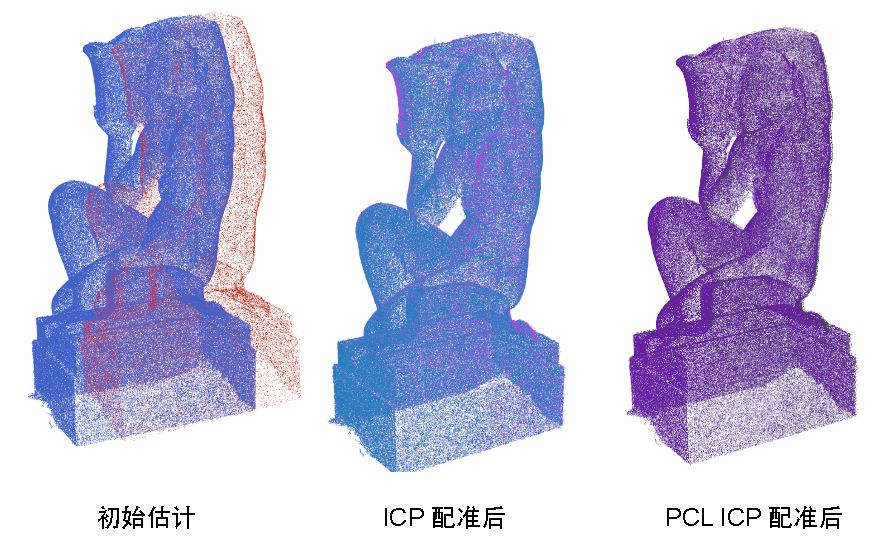
\includegraphics[width=0.8\textwidth]{3d-lidar-mapping/ch7-align-results.pdf}
	\caption{Alignment visualization: (Left) Initial pose, (Middle) Our ICP, (Right) PCL ICP}
	\label{fig:icp-align-results}
\end{figure}

Despite its simplicity, point-to-point ICP faces limitations in autonomous driving scenarios. The sparsity of LiDAR point clouds means consecutive scans rarely sample identical surface points. Matching discrete points directly (as in basic ICP) proves suboptimal. Subsequent sections address this through:
\begin{itemize}
	\item Multi-point correspondences (point-to-plane ICP)
	\item Distribution-based matching (NDT)
	\item Feature-level registration.
\end{itemize}

\subsection{Point-to-Line and Point-to-Plane ICP}
\subsubsection{Theoretical Foundations}
Point-to-line and point-to-plane ICP are direct extensions of the standard ICP method. Their principles are similar to the 2D point-to-line ICP introduced in the previous chapter, with the optimization variables extended to 3D space and derivatives handled using manifold representations. 

Following the definitions from the previous section, let's consider two point clouds $S_1$ and $S_2$ with transformation parameters $\mathbf{R}, \mathbf{t}$. For each transformed point $\mathbf{R} \mathbf{q}_i + \mathbf{t}$, instead of finding a single nearest neighbor $\mathbf{p}_i$, we find multiple nearest neighbors and fit either a plane or a line to them.

\paragraph{Point-to-Plane ICP}  
For plane fitting, assume the plane parameters are $(\mathbf{n},d) \in \mathbb{R}^4$, where $\mathbf{n}$ is the unit normal vector and $d$ is the intercept. For any point $\mathbf{p}$ on the plane:
\begin{equation}\label{key}
	\mathbf{n}^\top \mathbf{p} + d = 0.
\end{equation}
The signed distance from a point $\mathbf{q}_i$ to the plane is:
\begin{equation}\label{key}
	e_i = \mathbf{n}^\top (\mathbf{R} \mathbf{q}_i + \mathbf{t}) + d.
\end{equation}
Note that since $|\mathbf{n}|=1$, no normalization is needed. The derivatives with respect to $\mathbf{R}$ and $\mathbf{t}$ are:
\begin{equation}\label{key}
	\frac{\partial e_i}{\partial \mathbf{R}} = -\mathbf{n}^\top \mathbf{R} \mathbf{q}_i^\wedge, \quad \frac{\partial e_i}{\partial \mathbf{t}} = \mathbf{n}.
\end{equation}

\paragraph{Point-to-Line ICP}  
For line fitting, parameterize the line as:
\begin{equation}\label{key}
	\mathbf{p} = \mathbf{d} \tau + \mathbf{p}_0,
\end{equation}
where $\mathbf{d}$ is the unit direction vector, $\mathbf{p}_0$ is a point on the line, and $\tau$ is a scalar parameter. The perpendicular distance from $\mathbf{q}_i$ to the line is given by the cross product:
\begin{equation}\label{key}
	\mathbf{e}_i = \mathbf{d} \times (\mathbf{R} \mathbf{q}_i + \mathbf{t} - \mathbf{p}_0) = \mathbf{d}^\wedge (\mathbf{R} \mathbf{q}_i + \mathbf{t} - \mathbf{p}_0).
\end{equation}
The derivatives are:
\begin{equation}\label{key}
	\frac{\partial \mathbf{e}_i}{\partial \mathbf{R}} = -\mathbf{d}^\wedge \mathbf{R} \mathbf{q}_i^\wedge, \quad \frac{\partial \mathbf{e}_i}{\partial \mathbf{t}} = \mathbf{d}^\wedge.
\end{equation}

These derivatives are straightforward to derive, and we leave their complete derivation as an exercise for the reader.

\subsection{Point-to-Line ICP Implementation}
The point-to-line ICP follows the same principle as previous methods, with modifications to use line-based residuals. Below shows the key implementation differences:

\begin{lstlisting}[language=c++,caption=ch7/icp\_3d.cc]
std::for_each(std::execution::par_unseq, index.begin(), index.end(), [&](int idx) {
	auto q = ToVec3d(source_->points[idx]);
	Vec3d qs = pose * q;  // Transformed point
	std::vector<int> nn;
	kdtree_->GetClosestPoint(ToPointType(qs), nn, 5);  // 5 neighbors for line fitting
	
	if (nn.size() == 5) {
		std::vector<Vec3d> nn_eigen;
		for (int i = 0; i < 5; ++i) {
			nn_eigen.emplace_back(ToVec3d(target_->points[nn[i]]));
		}
		
		Vec3d direction, point_on_line;
		if (!math::FitLine(nn_eigen, point_on_line, direction, 
		options_.max_line_distance_)) {
			effect_pts[idx] = false;
			return;
		}
		
		Vec3d err = SO3::hat(direction) * (qs - point_on_line);
		
		if (err.norm() > options_.max_line_distance_) {
			effect_pts[idx] = false;
			return;
		}
		
		effect_pts[idx] = true;
		
		// Build 3x6 Jacobian
		Eigen::Matrix<double, 3, 6> J;
		J.block<3, 3>(0, 0) = -SO3::hat(direction) * pose.so3().matrix() * SO3::hat(q);
		J.block<3, 3>(0, 3) = SO3::hat(direction);
		
		jacobians[idx] = J;
		errors[idx] = err;
	} else {
		effect_pts[idx] = false;
	}
});
\end{lstlisting}

Key implementation notes:
\begin{itemize}
	\item Uses 5 nearest neighbors for line fitting
	\linebreak[1] \item Jacobian becomes 3×6 dimensional
	\linebreak[1] \item Residual becomes 3D vector (perpendicular distance components)
\end{itemize}

Benchmark results show comparable performance to point-to-point ICP:

\begin{lstlisting}[language=c++,caption=Terminal output]
I0130 16:46:41.100083 84155 icp_3d.cc:232] Aligning with point-to-line
I0130 16:46:41.109969 84155 icp_3d.cc:325] Iter 0 | Pose error: 0.0536 | Res: 11.360 | Eff: 44503 | Avg: 0.000255 | dx: 0.0431
I0130 16:46:41.118880 84155 icp_3d.cc:325] Iter 1 | Pose error: 0.0279 | Res: 3.6516 | Eff: 44515 | Avg: 8.20e-05 | dx: 0.0262
I0130 16:46:41.127648 84155 icp_3d.cc:325] Iter 2 | Pose error: 0.0143 | Res: 1.013 | Eff: 44515 | Avg: 2.28e-05 | dx: 0.0138
I0130 16:46:41.135840 84155 icp_3d.cc:325] Iter 3 | Pose error: 0.0073 | Res: 0.292 | Eff: 44515 | Avg: 6.58e-06 | dx: 0.00714
I0130 16:46:41.135859 84155 icp_3d.cc:333] Converged, dx = [0.00545, -0.00273, -0.00242, -0.000307, 0.00164, -0.00229]
E0130 16:46:41.135869 84155 test_icp.cc:96] ICP success. Pose: [0.0296, -0.0118, -0.0257, 0.999], [-0.0702, -0.1019, 0.00249]
I0130 16:46:41.186185 84155 sys_utils.h:32] ICP P2Line avg time: 157.942ms (1 runs)
\end{lstlisting}

Performance comparison:
\begin{itemize}
	\item \textbf{Accuracy}: Point-to-plane > Point-to-line ≈ Point-to-point
	\item \textbf{Efficiency}: All variants significantly outperform PCL's implementation
\end{itemize}

An important observation arises: Why limit ourselves to a single residual type? Modern approaches often:
\begin{enumerate}
	\item Classify local geometry (planar/linear) in the target cloud
	\item Dynamically select point-to-plane or point-to-line residuals
\end{enumerate}

This feature-adaptive approach, common in autonomous driving, will be explored later. First, we introduce another statistical registration method: NDT (Normal Distributions Transform).

\subsection{NDT Method}
\label{sec:ndt}
\subsubsection{Principles}
Whether point-to-line or point-to-plane ICP, their fundamental difference from standard ICP lies in registering points not to individual \textbf{points}, but to certain \textbf{statistical measures}. Point-to-plane ICP fits local points to planes, while point-to-line ICP fits them to lines. Extending this idea further: Why must we presuppose whether points form planes or lines? Why precisely determine surface/line parameters? We only need the \textbf{local statistics} of the point cloud for matching. The most basic statistical measures of a point set are its \textbf{mean} and \textbf{covariance}. Following this reasoning leads to the traditional NDT (Normal Distribution Transform) method \cite{Ulas2013,Saarinen2013}.

This section explains NDT principles using simplified notation, which differs slightly from the original NDT papers while maintaining theoretical consistency. The NDT workflow:

\begin{enumerate}
	\item Partition the target point cloud into voxels at a specified resolution.
	\item Compute Gaussian distributions for each voxel. Let $\boldsymbol{\mu}_k$ and $\boldsymbol{\Sigma}_k$ denote the mean and covariance of the $k$-th voxel.
	\item During registration, determine which voxel each transformed point occupies, then establish residuals between the point and the voxel's $\boldsymbol{\mu}_k, \boldsymbol{\Sigma}_k$.
	\item Iteratively refine the pose estimate using Gauss-Newton or Levenberg-Marquardt.
\end{enumerate}

The key step is \#3. For a source point $\mathbf{q}_i$ transformed by $\mathbf{R}, \mathbf{t}$ into a voxel with statistics $\boldsymbol{\mu}_i, \boldsymbol{\Sigma}_i$\footnote{In practice, pose errors may place points in adjacent voxels. Most NDT implementations search neighboring voxels to improve convergence.}, we define the voxel residual as:
\begin{equation}\label{key}
	\mathbf{e}_i = \mathbf{R} \mathbf{q}_i + \mathbf{t} - \boldsymbol{\mu}_i,
\end{equation}

The optimal $\mathbf{R}, \mathbf{t}$ solve a weighted least-squares problem:
\begin{equation}\label{key}
	(\mathbf{R},\mathbf{t})^* = \arg \min\limits_{\mathbf{R}, \mathbf{t}} \sum_{i} (\mathbf{e}_i^\top \boldsymbol{\Sigma}_i^{-1} \mathbf{e}_i) .
\end{equation}

From least-squares theory, this equivalently maximizes the probability of each point belonging to its voxel's distribution - a maximum likelihood estimation (MLE)\footnote{Readers unfamiliar should consult Chapter 6 of \textit{14 Lectures}.}:
\begin{equation}\label{key}
	(\mathbf{R},\mathbf{t})^* = \arg \max\limits_{\mathbf{R}, \mathbf{t}} \prod_{i} P(\mathbf{R} \mathbf{q}_i + \mathbf{t})
\end{equation}
Here, $\boldsymbol{\Sigma}^{-1}_i$ provides the weighting: tighter distributions demand closer alignment to $\boldsymbol{\mu}_i$, while dispersed distributions tolerate greater deviation.

The Gauss-Newton system becomes:
\begin{equation}\label{eq:ndt-normal-equation}
	\sum_{i} (\mathbf{J}_i^\top \boldsymbol{\Sigma}_i^{-1} \mathbf{J}_i) \Delta \mathbf{x} = -\sum_{i} \mathbf{J}_i^\top \boldsymbol{\Sigma}^{-1}_i \mathbf{e}_i,
\end{equation}
where $\Delta \mathbf{x}$ is the increment and $\mathbf{J}_i$ the Jacobian:
\begin{equation}\label{key}
	\frac{\partial \mathbf{e}_i}{\partial \mathbf{R}} = -\mathbf{R} \mathbf{q}_i^\wedge, \quad \frac{\partial \mathbf{e}_i}{\partial \mathbf{t}} = \mathbf{I}.
\end{equation}
Levenberg-Marquardt can enhance robustness.

\textbf{Note}: This derivation differs significantly from \cite{Magnusson2009}, aligning more closely with early 2D NDT \cite{Biber2003}. The core principles remain identical - the original formulation used trigonometric expressions before manifold optimization became prevalent in SLAM. We omit the uniform distribution component for clarity, as most implementations incorporate practical improvements \cite{Kung2021, Rapp2015}. Similarly, other algorithms in this book adapt original formulations to maintain consistent notation.

\subsubsection{Implementation}
The NDT implementation consists of two main components: voxel construction and registration. The NDT class internally maintains these voxels and their indices. The voxel construction process is similar to the grid method described in Chapter 5, but without requiring nearest neighbor search implementation. The core code is as follows:

\begin{lstlisting}[language=c++,caption=src/ch7/ndt\_3d.cc]
class Ndt3d {
	public:
	enum class NearbyType {
		CENTER,   // Consider only center
		NEARBY6,  // Up/down/left/right/front/back
	};
	
	using KeyType = Eigen::Matrix<int, 3, 1>;  // Voxel index
	struct VoxelData {
		VoxelData() {}
		VoxelData(size_t id) { idx_.emplace_back(id); }
		
		std::vector<size_t> idx_;      // Point indices in cloud
		Vec3d mu_ = Vec3d::Zero();     // Mean
		Mat3d sigma_ = Mat3d::Zero();  // Covariance
		Mat3d info_ = Mat3d::Zero();   // Inverse covariance
	};
	
	private:
	void BuildVoxels();
	
	/// Generate nearby grids based on neighbor type
	void GenerateNearbyGrids();
	
	CloudPtr target_ = nullptr;
	CloudPtr source_ = nullptr;
	
	Vec3d target_center_ = Vec3d::Zero();
	Vec3d source_center_ = Vec3d::Zero();
	Options options_;
	
	std::unordered_map<KeyType, VoxelData, hash_vec<3>> grids_;  // Voxel data
	std::vector<KeyType> nearby_grids_;                          // Nearby voxels
};

void Ndt3d::BuildVoxels() {
	assert(target_ != nullptr);
	assert(target_->empty() == false);
	
	/// Assign points to voxels
	std::vector<size_t> index(target_->size());
	std::iota(index.begin(), index.end(), 0);
	
	std::for_each(index.begin(), index.end(), [this](const size_t& idx) {
		auto pt = ToVec3d(target_->points[idx]);
		auto key = (pt * options_.inv_voxel_size_).cast<int>();
		grids_[key].idx_.emplace_back(idx);
	});
	
	/// Compute mean and covariance for each voxel
	std::for_each(std::execution::par_unseq, grids_.begin(), grids_.end(), [this](auto& v) {
		if (v.second.idx_.size() > options_.min_pts_in_voxel_) {
			// Minimum 3 points required
			math::ComputeMeanAndCov(v.second.idx_, v.second.mu_, v.second.sigma_,
			[this](const size_t& idx) { return ToVec3d(target_->points[idx]); });
			// Regularize covariance matrix
			v.second.info_ = (v.second.sigma_ + Mat3d::Identity() * 1e-3).inverse();
		}
	});
	
	/// Remove voxels with insufficient points
	for (auto iter = grids_.begin(); iter != grids_.end();) {
		if (iter->second.idx_.size() > options_.min_pts_in_voxel_) {
			iter++;
		} else {
			iter = grids_.erase(iter);
		}
	}
	
	LOG(INFO) << "voxels: " << grids_.size();
}

void Ndt3d::GenerateNearbyGrids() {
	nearby_grids_.clear();
	if (options_.nearby_type_ == NearbyType::CENTER) {
		nearby_grids_.emplace_back(KeyType::Zero());
	} else if (options_.nearby_type_ == NearbyType::NEARBY6) {
		nearby_grids_ = {KeyType(0, 0, 0),  KeyType(-1, 0, 0), KeyType(1, 0, 0), 
			KeyType(0, 1, 0), KeyType(0, -1, 0), KeyType(0, 0, -1), 
			KeyType(0, 0, 1)};
	}
}
\end{lstlisting}

\subsubsection{Voxel Neighbor Selection}
Users can configure the voxel neighbor search strategy. We can either use only the center voxel or include its six adjacent voxels as neighbors. For any voxel containing at least three points, we compute its mean and covariance. 

Note that in simulation scenarios, multiple points may share identical coordinates along certain axes, causing zero values in the covariance matrix diagonal. Similarly, when points within a voxel approximate a plane or line, the covariance matrix may become singular. Therefore, we add a small regularization term (1e-3) to the diagonal before matrix inversion to ensure numerical stability.

The NDT registration implementation:

\begin{lstlisting}[language=c++,caption=src/ch7/ndt\_3d.cc]
bool Ndt3d::AlignNdt(SE3& init_pose) {
	LOG(INFO) << "Aligning with NDT";
	assert(!grids_.empty());
	
	SE3 pose = init_pose;
	if (options_.remove_centroid_) {
		pose.translation() = target_center_ - source_center_;  // Initialize translation
		LOG(INFO) << "Initial translation: " << pose.translation().transpose();
	}
	
	// Precompute point indices
	int num_residual_per_point = options_.nearby_type_ == NearbyType::NEARBY6 ? 7 : 1;
	std::vector<int> index(source_->size());
	std::iota(index.begin(), index.end(), 0);
	
	for (int iter = 0; iter < options_.max_iteration_; ++iter) {
		// Parallel computation buffers
		std::vector<bool> effect_pts(index.size() * num_residual_per_point, false);
		std::vector<Eigen::Matrix<double, 3, 6>> jacobians(effect_pts.size());
		std::vector<Vec3d> errors(effect_pts.size());
		std::vector<Mat3d> infos(effect_pts.size());
		
		// Parallel residual computation
		std::for_each(std::execution::par_unseq, index.begin(), index.end(), [&](int idx) {
			Vec3d qs = pose * ToVec3d(source_->points[idx]);
			Vec3i base_key = (qs * options_.inv_voxel_size_).cast<int>();
			
			for (int i = 0; i < nearby_grids_.size(); ++i) {
				Vec3i key = base_key + nearby_grids_[i];
				int buffer_idx = idx * num_residual_per_point + i;
				
				if (auto it = grids_.find(key); it != grids_.end()) {
					const auto& v = it->second;
					Vec3d e = qs - v.mu_;
					double res = e.transpose() * v.info_ * e;
					
					if (std::isnan(res) || res > options_.res_outlier_th_) {
						continue;  // Reject outliers
					}
					
					// Build residual and Jacobian
					jacobians[buffer_idx].block<3,3>(0,0) = -pose.so3().matrix() * SO3::hat(q);
					jacobians[buffer_idx].block<3,3>(0,3) = Mat3d::Identity();
					errors[buffer_idx] = e;
					infos[buffer_idx] = v.info_;
					effect_pts[buffer_idx] = true;
				}
			}
		});
		
		// Accumulate Hessian and error
		Mat6d H = Mat6d::Zero();
		Vec6d err = Vec6d::Zero();
		double total_res = 0;
		int effective_num = 0;
		
		for (int i = 0; i < effect_pts.size(); ++i) {
			if (!effect_pts[i]) continue;
			
			H += jacobians[i].transpose() * infos[i] * jacobians[i];
			err -= jacobians[i].transpose() * infos[i] * errors[i];
			total_res += errors[i].transpose() * infos[i] * errors[i];
			effective_num++;
		}
		
		if (effective_num < options_.min_effective_pts_) {
			LOG(WARNING) << "Insufficient correspondences: " << effective_num;
			return false;
		}
		
		// Update pose
		Vec6d dx = H.ldlt().solve(err);
		pose.so3() = pose.so3() * SO3::exp(dx.head<3>());
		pose.translation() += dx.tail<3>();
		
		LOG(INFO) << "Iter " << iter << " | Res: " << total_res 
		<< " | Eff: " << effective_num
		<< " | Avg: " << total_res/effective_num
		<< " | dx: " << dx.norm();
		
		if (gt_set_) {
			LOG(INFO) << "Pose error: " << (gt_pose_.inverse() * pose).log().norm();
		}
		
		if (dx.norm() < options_.eps_) break;
	}
	
	init_pose = pose;
	return true;
}
\end{lstlisting}

Key implementation notes:
\begin{itemize}
	\item Supports configurable neighbor search (center-only or 6-adjacent)
	\item Parallelized residual computation using C++17 execution policies
	\item Regularized covariance matrices (1e-3) for numerical stability
	\item Outlier rejection based on Mahalanobis distance threshold
	\item Efficient LDLT decomposition for solving the linear system
\end{itemize}

The overall workflow remains consistent with our previous discussion, though readers may incorporate additional convergence checks as needed. The inclusion of covariance matrices imposes constraints during Gauss-Newton iterations, accelerating convergence\footnote{Similar covariance constraints could be applied in point-to-plane ICP, e.g., prioritizing errors along plane normals rather than uniform optimization.}. When executing the test program, readers will observe significantly faster performance from this NDT implementation:

\begin{lstlisting}[language=sh,caption=Terminal output:]
I0130 17:48:05.746295 88880 ndt_3d.cc:69] Aligning with NDT
I0130 17:48:05.746309 88880 ndt_3d.cc:75] Initial translation: -0.0565748 -0.122053 0.0288451
I0130 17:48:05.748436 88880 ndt_3d.cc:168] Iter 0 | Res: 136282 | Eff: 44120 | Avg: 3.0889 | dx: 0.0323 [0.0212, -0.0005, -0.0209, -0.0078, 0.0069, -0.0071]
I0130 17:48:05.748458 88880 ndt_3d.cc:178] Pose error: 0.065853
[...]
I0130 17:48:05.754640 88880 ndt_3d.cc:182] Converged, dx = [0.0069, -0.0035, -0.0049, -0.0005, 0.0021, -0.0031]
E0130 17:48:05.754648 88880 test_icp.cc:121] NDT success. Pose: [0.0267, -0.0049, -0.0222, 0.9994], [-0.0713, -0.1045, 0.0086]
I0130 17:48:05.758247 88880 sys_utils.h:32] NDT avg time: 20.9043ms (1 runs)
[...]
I0130 17:44:52.928387 88363 test_icp.cc:167] PCL NDT pose error: 0.201841
I0130 17:44:52.928720 88363 sys_utils.h:32] PCL NDT avg time: 250.998ms (1 runs)
\end{lstlisting}

Performance benchmarks show:
\begin{itemize}
	\item \textbf{Center-voxel mode}: 10x faster than PCL implementation
	\item \textbf{6-neighbor mode}: 3-4x faster than PCL
	\item \textbf{Dense point clouds}: Prefer center-voxel for efficiency
	\item \textbf{Sparse point clouds}: Include neighboring voxels for robustness
\end{itemize}

NDT's elegant formulation and general applicability (unlike ICP's need for geometric assumptions) have established it as a standard benchmark for registration algorithms. However, two fundamental challenges persist:

\begin{itemize}
	\item \textbf{Initial guess dependency}: Like all registration methods, poor initialization may place points in incorrect voxels, leading to misalignment.
	\item \textbf{Voxel size sensitivity}: The algorithm's discretization introduces a critical hyperparameter:
	\begin{itemize}
		\item Oversized voxels lose geometric fidelity in dense clouds
		\item Undersized voxels contain insufficient points for meaningful statistics
	\end{itemize}
\end{itemize}

\textbf{Practical recommendation}: Always conduct voxel size analysis during implementation, as this parameter profoundly impacts registration accuracy while lacking universal optimal values. The appropriate scale depends entirely on the scene's spatial characteristics and point density.

\subsection{Comparative Analysis of Registration Methods vs. PCL Implementations}
\begin{figure}[!t]
	\centering
	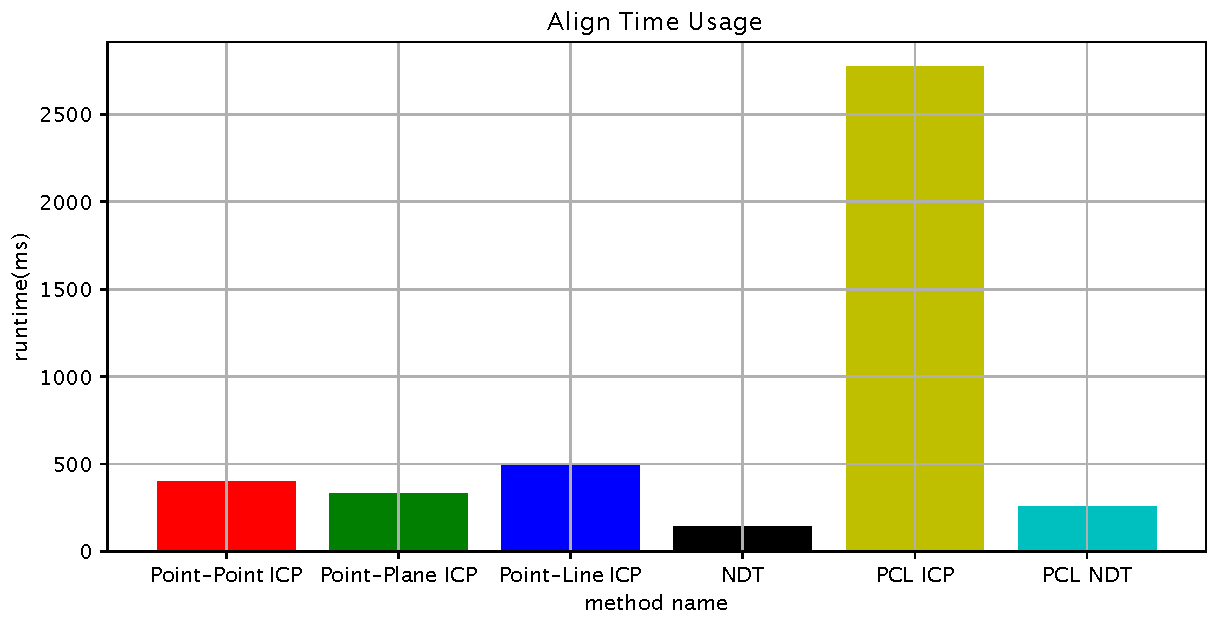
\includegraphics[width=0.6\textwidth]{resources/3d-lidar-mapping/align_time_usage.pdf}
	\caption{Computation time comparison across registration methods}
	\label{fig:align-time-usage}
\end{figure}

\begin{figure}[!t]
	\centering
	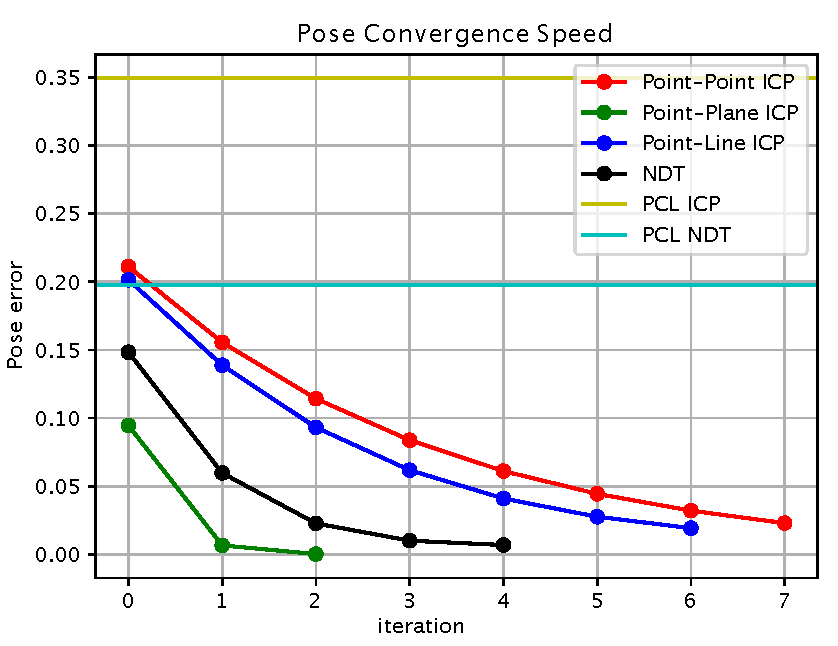
\includegraphics[width=0.6\textwidth]{resources/3d-lidar-mapping/pose_conv_speed.pdf}
	\caption{Pose convergence curves of different registration methods}
	\label{fig:pose-conv-speed}
\end{figure}

Using the EPFL dataset provided in this chapter, we evaluate the temporal efficiency and accuracy metrics of various registration methods. Our current implementation facilitates horizontal comparison of:
\begin{enumerate}
	\item Our point-to-point ICP (Sec. 7.2.1);
	\item Our point-to-plane ICP (Sec. 7.2.2); 
	\item Our point-to-line ICP (Sec. 7.2.3);
	\item Our NDT implementation (Sec. 7.3);
	\item PCL's ICP implementation;
	\item PCL's NDT implementation.
\end{enumerate}

Figures~\ref{fig:align-time-usage} and~\ref{fig:pose-conv-speed} present the computational time and error convergence profiles respectively. Since PCL implementations only output final poses without intermediate iterations, their errors are represented as horizontal lines. Key observations from our benchmark:

\begin{itemize}
	\item \textbf{Point-to-plane ICP} achieves the highest pose accuracy with fastest convergence for small models like EPFL datasets
	\item \textbf{NDT} demonstrates competitive speed but slightly inferior final accuracy compared to point-to-plane ICP
	\item \textbf{Basic point-to-point ICP} shows relatively poor performance, serving mainly as a baseline
\end{itemize}

Further subdivision by nearest neighbor methods (K-dTree vs voxel-based) reveals additional performance variations. We encourage readers to conduct extended comparisons, though our experiments already establish a framework for evaluating registration algorithms. 

\textbf{Critical Note}: Small model performance doesn't directly translate to large-scale scenarios. For compact models with smooth surfaces (like EPFL), point-to-plane ICP benefits from rich geometric constraints. NDT's effectiveness becomes voxel-size dependent - overly coarse voxels may prevent optimal convergence. However, autonomous driving scenarios present fundamentally different characteristics:

\begin{itemize}
	\item Sparse point clouds with large structures
	\item Higher noise levels
	\item Reduced surface completeness
\end{itemize}

Algorithm selection must therefore consider specific application contexts rather than relying on singular dataset performance. The optimal method varies significantly between precision small-object registration and large-scale noisy environment mapping.

\section{Direct Method LiDAR Odometry}
With registration methods like ICP and NDT, we can align multiple point clouds to form local maps and ultimately build a LiDAR odometry module. The simplest approach is to consecutively apply scan-to-scan matching between consecutive frames. In 3D SLAM, point clouds can be easily merged - we can compose a local map from recent scans and register the current frame against this map. This feature-free approach is called direct LiDAR odometry. Depending on the registration method used, we can implement various direct odometry solutions based on different ICP or NDT variants, as shown in the left portion of Fig.~\ref{fig:lo-pipeline}.

For higher precision with slightly more computation, we can enhance the NDT implementation at the voxel level. Instead of concatenating historical point clouds into a local map, we can incrementally update the Gaussian distributions within NDT voxels using newly registered points. This incremental NDT approach avoids reconstructing the entire NDT structure or KD-trees for each frame, enabling highly efficient implementation. Below we implement both approaches and compare their computational performance.

\begin{figure}[!thp]
	\centering
	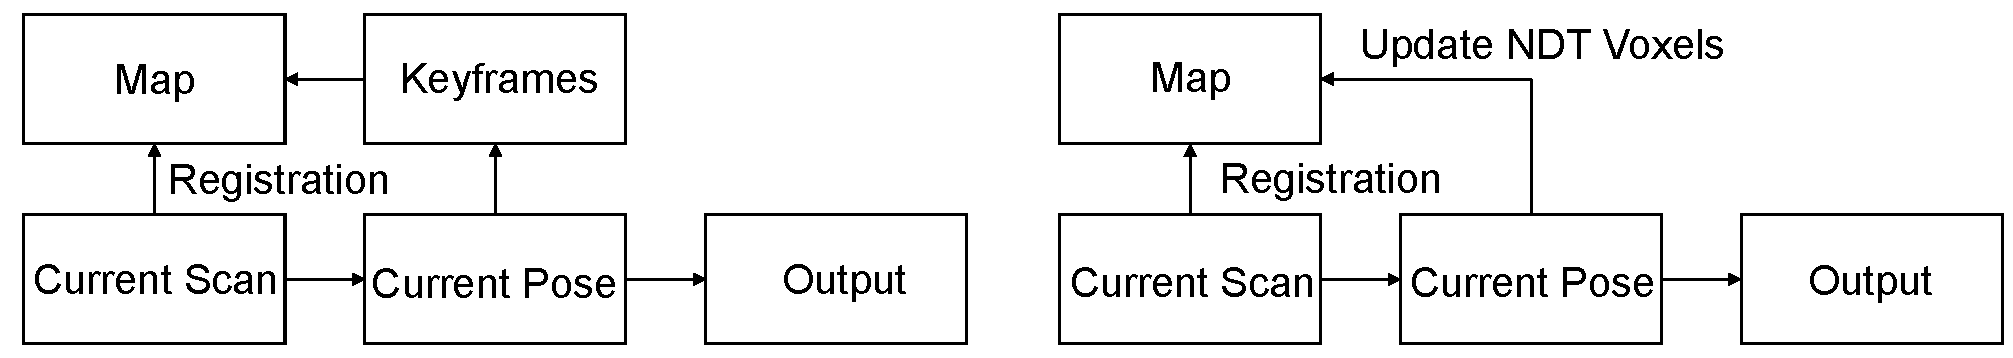
\includegraphics[width=1.0\textwidth]{resources/3d-lidar-mapping/lo-pipeline.pdf}
	\caption{Two implementation approaches for LiDAR odometry.}
	\label{fig:lo-pipeline}
\end{figure}

\subsection{Building LiDAR Odometry with NDT}
\label{sec:ndt-odom}
We first implement the LiDAR odometry following the initial approach. This odometry maintains a local map composed of multiple scans, registers them collectively, and uses the NDT alignment from Section~\ref{sec:ndt} to estimate the current frame's pose. The core implementation is as follows:

\begin{lstlisting}[language=c++, caption=src/ch7/direct\_ndt\_lo.cc]
class DirectNDTLO {
	public:
	struct Options {
		Options() {}
		double kf_distance_ = 0.5;            // Keyframe distance threshold
		double kf_angle_deg_ = 30;            // Rotation threshold
		int num_kfs_in_local_map_ = 30;       // Local map keyframe capacity  
		bool use_pcl_ndt_ = true;            // Use our NDT or PCL's NDT
		bool display_realtime_cloud_ = true;  // Enable real-time visualization
		
		Ndt3d::Options ndt3d_options_;       // NDT3D configuration
	};
	
	DirectNDTLO(Options options = Options()) : options_(options) {
		if (options_.display_realtime_cloud_) {
			viewer_ = std::make_shared<PCLMapViewer>(0.5);
		}
		
		ndt_ = Ndt3d(options_.ndt3d_options_);
		
		// Configure PCL NDT
		ndt_pcl_.setResolution(1.0);
		ndt_pcl_.setStepSize(0.1);
		ndt_pcl_.setTransformationEpsilon(0.01);
	}
	
	/**
	* Process a new point cloud scan
	* @param scan  Current frame point cloud  
	* @param pose  Estimated pose (output)
	*/
	void AddCloud(CloudPtr scan, SE3& pose);
	
	private:
	/// Align scan with local map
	SE3 AlignWithLocalMap(CloudPtr scan);
	
	/// Keyframe decision logic
	bool IsKeyframe(const SE3& current_pose);
	
	private:
	Options options_;
	CloudPtr local_map_ = nullptr;
	std::deque<CloudPtr> scans_in_local_map_;
	std::vector<SE3> estimated_poses_;  // Estimated trajectory
	SE3 last_kf_pose_;                  // Last keyframe pose
	
	pcl::NormalDistributionsTransform<PointType, PointType> ndt_pcl_;
	Ndt3d ndt_;
};

void DirectNDTLO::AddCloud(CloudPtr scan, SE3& pose) {
	if (local_map_ == nullptr) {
		// Initialize with first frame
		local_map_.reset(new PointCloudType);
		*local_map_ += *scan;
		pose = SE3();
		last_kf_pose_ = pose;
		
		if (options_.use_pcl_ndt_) {
			ndt_pcl_.setInputTarget(local_map_);
		} else {
			ndt_.SetTarget(local_map_);
		}
		return;
	}
	
	// Align scan with local map
	pose = AlignWithLocalMap(scan);
	CloudPtr scan_world(new PointCloudType);
	pcl::transformPointCloud(*scan, *scan_world, pose.matrix().cast<float>());
	
	if (IsKeyframe(pose)) {
		last_kf_pose_ = pose;
		
		// Update local map
		scans_in_local_map_.emplace_back(scan_world);
		if (scans_in_local_map_.size() > options_.num_kfs_in_local_map_) {
			scans_in_local_map_.pop_front();
		}
		
		local_map_.reset(new PointCloudType);
		for (auto& scan : scans_in_local_map_) {
			*local_map_ += *scan;
		}
		
		if (options_.use_pcl_ndt_) {
			ndt_pcl_.setInputTarget(local_map_);
		} else {
			ndt_.SetTarget(local_map_);
		}
	}
}

SE3 DirectNDTLO::AlignWithLocalMap(CloudPtr scan) {
	if (options_.use_pcl_ndt_) {
		ndt_pcl_.setInputSource(scan);
	} else {
		ndt_.SetSource(scan);
	}
	
	SE3 guess;
	bool align_success = true;
	
	if (estimated_poses_.size() < 2) {
		// Initial alignment without motion model
		if (options_.use_pcl_ndt_) {
			pcl::PointCloud<PointType> output;
			ndt_pcl_.align(output, guess.matrix().cast<float>());
			guess = Mat4dToSE3(ndt_pcl_.getFinalTransformation().cast<double>());
		} else {
			align_success = ndt_.AlignNdt(guess);
		}
	} else {
		// Motion model prediction from last two poses
		SE3 T1 = estimated_poses_.back();
		SE3 T2 = estimated_poses_[estimated_poses_.size() - 2];
		guess = T1 * (T2.inverse() * T1);
		
		if (options_.use_pcl_ndt_) {
			pcl::PointCloud<PointType> output;
			ndt_pcl_.align(output, guess.matrix().cast<float>());
			guess = Mat4dToSE3(ndt_pcl_.getFinalTransformation().cast<double>());
		} else {
			align_success = ndt_.AlignNdt(guess);
		}
	}
	
	LOG(INFO) << "Estimated pose - t: " << guess.translation().transpose() 
	<< ", q: " << guess.so3().unit_quaternion().coeffs().transpose();
	
	if (options_.use_pcl_ndt_) {
		LOG(INFO) << "Transformation probability: " << ndt_pcl_.getTransformationProbability();
	}
	
	estimated_poses_.emplace_back(guess);
	return guess;
}
\end{lstlisting}

This basic odometry continuously aligns incoming scans against a local map using NDT registration. Users can select either PCL's NDT or our custom implementation. Keyframes are selected based on distance or rotation thresholds, with recent keyframes aggregated into a local map serving as the NDT target. For alignment initialization, we employ a motion model derived from the relative movement of the last two frames. The system provides real-time visualization through a PCL-based 3D viewer and saves the merged point cloud as a PCD file upon completion.

The test program for this section is shown below, where gflags can specify whether to use PCL's NDT implementation and the number of nearest neighbors for our NDT:

\begin{lstlisting}[language=c++,caption=src/ch7/test/test_ndt_lo.cc]
	/// This program demonstrates NDT-based LiDAR Odometry using ULHK dataset
	/// When using PCL NDT, it rebuilds the NDT tree
	DEFINE_string(bag_path, "./dataset/sad/ulhk/test2.bag", "path to rosbag");
	DEFINE_string(dataset_type, "ULHK", "NCLT/ULHK/KITTI/WXB_3D");  // Dataset type
	DEFINE_bool(use_pcl_ndt, false, "use pcl ndt to align?");
	DEFINE_bool(use_ndt_nearby_6, false, "use ndt nearby 6?");
	DEFINE_bool(display_map, true, "display map?");
	
	int main(int argc, char** argv) {
		sad::RosbagIO rosbag_io(fLS::FLAGS_bag_path, sad::Str2DatasetType(FLAGS_dataset_type));
		
		sad::DirectNDTLO::Options options;
		options.use_pcl_ndt_ = fLB::FLAGS_use_pcl_ndt;
		options.ndt3d_options_.nearby_type_ =
		FLAGS_use_ndt_nearby_6 ? sad::Ndt3d::NearbyType::NEARBY6 : sad::Ndt3d::NearbyType::CENTER;
		options.display_realtime_cloud_ = FLAGS_display_map;
		sad::DirectNDTLO ndt_lo(options);
		
		rosbag_io
		.AddAutoPointCloudHandle([&ndt_lo](sensor_msgs::PointCloud2::Ptr msg) -> bool {
			sad::common::Timer::Evaluate(
			[&]() {
				SE3 pose;
				ndt_lo.AddCloud(sad::VoxelCloud(sad::PointCloud2ToCloudPtr(msg)), pose);
			},
			"NDT registration");
			return true;
		})
		.Go();
		
		if (FLAGS_display_map) {
			// Save the generated map
			ndt_lo.SaveMap("./data/ch7/map.pcd");
		}
		
		sad::common::Timer::PrintAll();
		LOG(INFO) << "done.";
		
		return 0;
	}
\end{lstlisting}

To run this program, readers need to download two test datasets from ULHK, with paths configurable via gflags. Compile and run with:

\begin{lstlisting}[language=sh,caption=Terminal command:]
	bin/test_ndt_lo 
\end{lstlisting}

You should see results similar to Fig.~\ref{fig:lo-map} (colors may vary - book illustrations typically use white background for printing). Upon completion, the Timer class prints algorithm efficiency:

\begin{lstlisting}[language=sh,caption=Terminal output:]
	I0131 10:51:49.840482 102707 timer.cc:16] >>> ===== Printing run time =====
	I0131 10:51:49.840484 102707 timer.cc:18] > [ NDT registration ] average time usage: 36.349 ms , called times: 3178
	I0131 10:51:49.840495 102707 timer.cc:23] >>> ===== Printing run time end =====
	I0131 10:51:49.840497 102707 test_ndt_lo.cc:56] done.
\end{lstlisting}

With visualization disabled, our NDT odometry processes each frame in about 15ms (18ms when using 6 nearest neighbors), while PCL's NDT takes about 85ms. Readers can benchmark both implementations on their own machines. The number of nearest neighbors affects registration efficiency, but isn't the dominant factor in the full odometry pipeline - merging local maps and constructing voxels/KD-trees for these maps consume most computational resources.

\begin{figure}[!t]
	\centering
	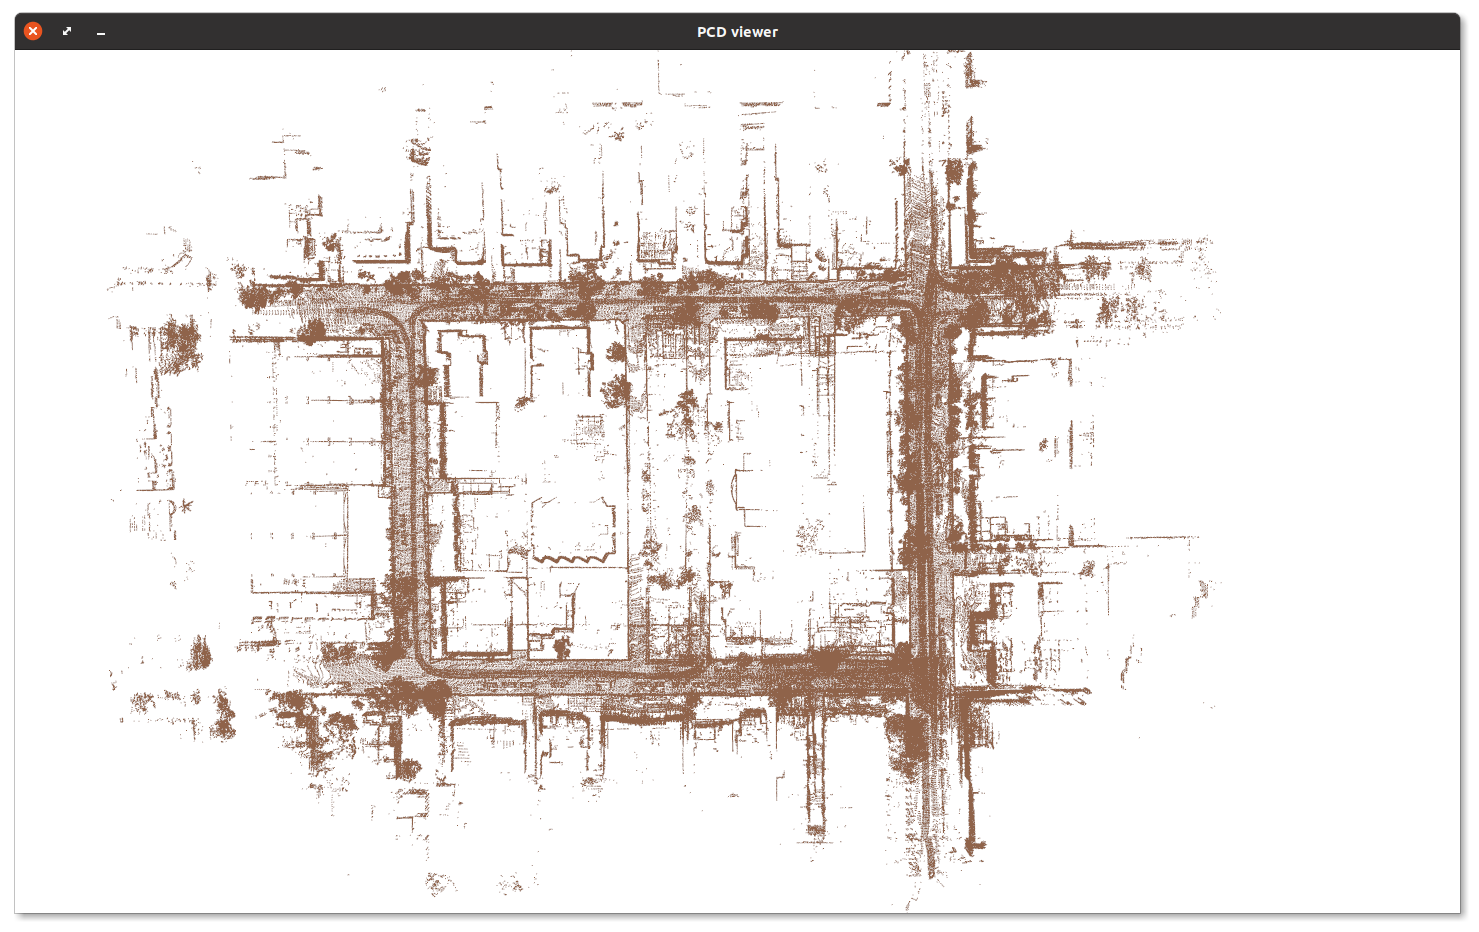
\includegraphics[width=1.0\textwidth]{resources/3d-lidar-mapping/ch7-lo-map}
	\caption{Point cloud map generated by our odometry, using ULHK dataset.}
	\label{fig:lo-map}
\end{figure}

Key reasons our NDT odometry outperforms PCL's implementation:
\begin{enumerate}
	\item While NDT is voxel-based, PCL's implementation still requires KD-trees for nearest neighbor searches. The time spent building KD-trees for local maps during scan-to-map registration is non-negligible. Our implementation directly uses voxel neighbors for faster lookups.
	\item We parallelize residual and Jacobian calculations during registration, significantly speeding up the process compared to PCL's serial implementation.
\end{enumerate}

However, the current LO pipeline has room for improvement. For example, when adding keyframes, we currently rebuild the entire local map and reset all NDT voxels. While faster than rebuilding KD-trees, this could be optimized further by incrementally updating voxels with new scan data while automatically discarding outdated voxels through a time-based queue - an approach we call \textbf{Incremental NDT}. We'll implement this next and compare its performance with the current method.

\subsection{Incremental NDT Odometry}
\label{sec:inc-ndt}
\subsubsection{Principles of Incremental Updates}
Implementing incremental NDT odometry raises two key challenges: maintaining dynamically growing voxels and determining how to update Gaussian parameters within each voxel. We first address the problem of updating statistical estimates within individual voxels. Specifically, given an existing Gaussian distribution estimated from historical points in a voxel, how should we update the distribution parameters when new points are added? This derivation requires basic probability theory.

\paragraph{Incremental Update of Gaussian Distribution}
Consider a voxel containing $m$ historical points with Gaussian parameters $\boldsymbol{\mu}_H, \boldsymbol{\Sigma}_H$. When adding $n$ new points with statistics $\boldsymbol{\mu}_A, \boldsymbol{\Sigma}_A$, we derive the updated distribution $\boldsymbol{\mu}, \boldsymbol{\Sigma}$. Let historical points be $\mathbf{x}_1, \ldots, \mathbf{x}_m$ and new points $\mathbf{y}_1, \ldots, \mathbf{y}_n$.

The mean update is straightforward:
\begin{equation}\label{key}
	\boldsymbol{\mu} = \frac{\sum_{i=1}^m \mathbf{x}_i + \sum_{j=1}^n \mathbf{y}_j}{m+n} = \frac{m \boldsymbol{\mu}_H + n\boldsymbol{\mu}_A}{m+n}.
\end{equation}

For covariance (ignoring Bessel's correction), we start with the sample covariance definition:
\begin{equation}\label{eq:7.18}
	\boldsymbol{\Sigma} = \frac{1}{m+n} \left( \sum_{i=1}^{m} (\mathbf{x}_i - \boldsymbol{\mu})(\mathbf{x}_i - \boldsymbol{\mu})^\top + \sum_{j=1}^{n} (\mathbf{y}_j - \boldsymbol{\mu})(\mathbf{y}_j - \boldsymbol{\mu})^\top \right).
\end{equation}

Expanding the first term using $\mathbf{x}_i - \boldsymbol{\mu} = (\mathbf{x}_i - \boldsymbol{\mu}_H) + (\boldsymbol{\mu}_H - \boldsymbol{\mu})$:
\begin{align}\label{key}
	\sum_{i=1}^{m} (\mathbf{x}_i - \boldsymbol{\mu})(\mathbf{x}_i - \boldsymbol{\mu})^\top &= \sum_{i=1}^{m} \left[ (\mathbf{x}_i - \boldsymbol{\mu}_H) + (\boldsymbol{\mu}_H - \boldsymbol{\mu}) \right] \left[ (\mathbf{x}_i - \boldsymbol{\mu}_H) + (\boldsymbol{\mu}_H - \boldsymbol{\mu}) \right]^\top \\
	&= m\boldsymbol{\Sigma}_H + \sum_{i=1}^m (\mathbf{x}_i - \boldsymbol{\mu}_H)(\boldsymbol{\mu}_H - \boldsymbol{\mu})^\top \\
	&\quad + \sum_{i=1}^m (\boldsymbol{\mu}_H - \boldsymbol{\mu})(\mathbf{x}_i - \boldsymbol{\mu}_H)^\top + m(\boldsymbol{\mu}_H - \boldsymbol{\mu})(\boldsymbol{\mu}_H - \boldsymbol{\mu})^\top.
\end{align}

The cross terms vanish since:
\begin{equation}\label{key}
	\sum_{i=1}^m (\mathbf{x}_i - \boldsymbol{\mu}_H) (\boldsymbol{\mu}_H - \boldsymbol{\mu})^\top = \left(\sum_{i=1}^m \mathbf{x}_i - m\boldsymbol{\mu}_H\right)(\boldsymbol{\mu}_H - \boldsymbol{\mu})^\top = \mathbf{0}.
\end{equation}

Thus we obtain:
\begin{equation}\label{key}
	\sum_{i=1}^{m} (\mathbf{x}_i - \boldsymbol{\mu})(\mathbf{x}_i - \boldsymbol{\mu})^\top = m \left(\boldsymbol{\Sigma}_H + (\boldsymbol{\mu}_H - \boldsymbol{\mu})(\boldsymbol{\mu}_H - \boldsymbol{\mu})^\top\right).
\end{equation}

Similarly for the new points:
\begin{equation}\label{key}
	\sum_{j=1}^{n} (\mathbf{y}_j - \boldsymbol{\mu})(\mathbf{y}_j - \boldsymbol{\mu})^\top = n \left(\boldsymbol{\Sigma}_A + (\boldsymbol{\mu}_A - \boldsymbol{\mu})(\boldsymbol{\mu}_A - \boldsymbol{\mu})^\top\right).
\end{equation}

The final covariance update formula becomes:
\begin{equation}\label{key}
	\boldsymbol{\Sigma} = \frac{m \left(\boldsymbol{\Sigma}_H + \Delta\boldsymbol{\mu}_H \Delta\boldsymbol{\mu}_H^\top\right) + n \left(\boldsymbol{\Sigma}_A + \Delta\boldsymbol{\mu}_A \Delta\boldsymbol{\mu}_A^\top\right)}{m+n}
\end{equation}
where $\Delta\boldsymbol{\mu}_H = \boldsymbol{\mu}_H - \boldsymbol{\mu}$ and $\Delta\boldsymbol{\mu}_A = \boldsymbol{\mu}_A - \boldsymbol{\mu}$. This formula enables efficient incremental updates of NDT voxel statistics.

\subsection{Incremental NDT Odometry}
\label{sec:inc-ndt}
\subsubsection{Incremental Voxel Maintenance}
Beyond updating Gaussian distributions within voxels, the voxel structure itself must dynamically expand as the vehicle moves. However, for long-term odometry operation, we must limit the total number of voxels (e.g., maintaining around 100,000 voxels) by periodically removing older ones. This requires implementing a least recently used (LRU) cache mechanism. We maintain a queue where recently updated voxels move to the front, while voxels exceeding capacity are removed from the back.

The implementation follows:

\begin{lstlisting}[language=c++,caption=src/ch7/ndt_inc.h]
	class IncNdt3d {
		public:
		enum class NearbyType {
			CENTER,   // Center voxel only
			NEARBY6,  // 6 adjacent voxels
		};
		
		using KeyType = Eigen::Matrix<int, 3, 1>;  // Voxel index
		
		/// Voxel data structure
		struct VoxelData {
			VoxelData() {}
			VoxelData(const Vec3d& pt) {
				pts_.emplace_back(pt);
				num_pts_ = 1;
			}
			
			void AddPoint(const Vec3d& pt) {
				pts_.emplace_back(pt);
				if (!ndt_estimated_) {
					num_pts_++;
				}
			}
			
			std::vector<Vec3d> pts_;       // Buffered points
			Vec3d mu_ = Vec3d::Zero();     // Mean
			Mat3d sigma_ = Mat3d::Zero();  // Covariance
			Mat3d info_ = Mat3d::Zero();   // Inverse covariance
			
			bool ndt_estimated_ = false;  // Whether Gaussian parameters are estimated
			int num_pts_ = 0;            // Total accumulated points
		};
		
		/// Add point cloud to voxels
		void AddCloud(CloudPtr cloud_world);
		
		/// NDT alignment using Gauss-Newton
		bool AlignNdt(SE3& init_pose);
		
		private:
		/// Update voxel statistics
		void UpdateVoxel(VoxelData& v);
		
		CloudPtr source_ = nullptr;
		Options options_;
		
		using KeyAndData = std::pair<KeyType, VoxelData>;
		std::list<KeyAndData> data_;  // LRU cache with actual data
		std::unordered_map<KeyType, std::list<KeyAndData>::iterator, hash_vec<3>> grids_;  // Hashmap for fast lookup
		std::vector<KeyType> nearby_grids_;  // Nearby voxel offsets
	};
\end{lstlisting}

The IncNdt3d class maintains voxel data in a doubly-linked list (for LRU management) while using a hashmap for O(1) access. When new points are added, we update voxel statistics and maintain the cache:

\begin{lstlisting}[language=c++,caption=src/ch7/ndt\_inc.cc]
	void IncNdt3d::AddCloud(CloudPtr cloud_world) {
		std::set<KeyType, less_vec<3>> active_voxels;  // Track updated voxels
		for (const auto& p : cloud_world->points) {
			auto pt = ToVec3d(p);
			auto key = (pt * options_.inv_voxel_size_).cast<int>();
			auto iter = grids_.find(key);
			
			if (iter == grids_.end()) {
				// New voxel
				data_.push_front({key, {pt}});
				grids_.insert({key, data_.begin()});
				
				if (data_.size() >= options_.capacity_) {
					// Remove oldest voxel
					grids_.erase(data_.back().first);
					data_.pop_back();
				}
			} else {
				// Existing voxel - add point and update LRU
				iter->second->second.AddPoint(pt);
				data_.splice(data_.begin(), data_, iter->second);
				iter->second = data_.begin();
			}
			
			active_voxels.emplace(key);
		}
		
		// Parallel voxel updates
		std::for_each(std::execution::par_unseq, active_voxels.begin(), active_voxels.end(),
		[this](const auto& key) { UpdateVoxel(grids_[key]->second); });
	}
	
	void IncNdt3d::UpdateVoxel(VoxelData& v) {
		if (v.ndt_estimated_ && v.num_pts_ > options_.max_pts_in_voxel_) {
			return;  // Skip if already well-estimated
		}
		
		if (!v.ndt_estimated_ && v.pts_.size() > options_.min_pts_in_voxel_) {
			// Initial estimation for new voxel
			math::ComputeMeanAndCov(v.pts_, v.mu_, v.sigma_, [](const Vec3d& p) { return p; });
			v.info_ = (v.sigma_ + Mat3d::Identity() * 1e-3).inverse();
			v.ndt_estimated_ = true;
			v.pts_.clear();
		} 
		else if (v.ndt_estimated_ && v.pts_.size() > options_.min_pts_in_voxel_) {
			// Incremental update for existing voxel
			Vec3d cur_mu, new_mu;
			Mat3d cur_var, new_var;
			math::ComputeMeanAndCov(v.pts_, cur_mu, cur_var, [](const Vec3d& p) { return p; });
			math::UpdateMeanAndCov(v.num_pts_, v.pts_.size(), v.mu_, v.sigma_, 
			cur_mu, cur_var, new_mu, new_var);
			
			v.mu_ = new_mu;
			v.sigma_ = new_var;
			v.num_pts_ += v.pts_.size();
			v.pts_.clear();
			
			// Regularize covariance
			Eigen::JacobiSVD svd(v.sigma_, Eigen::ComputeFullU | Eigen::ComputeFullV);
			Vec3d lambda = svd.singularValues();
			if (lambda[1] < lambda[0] * 1e-3) lambda[1] = lambda[0] * 1e-3;
			if (lambda[2] < lambda[0] * 1e-3) lambda[2] = lambda[0] * 1e-3;
			
			Mat3d inv_lambda = Vec3d(1.0/lambda[0], 1.0/lambda[1], 1.0/lambda[2]).asDiagonal();
			v.info_ = svd.matrixV() * inv_lambda * svd.matrixU().transpose();
		}
	}
\end{lstlisting}

Key features:
\begin{itemize}
	\item Each voxel tracks whether its Gaussian parameters have been estimated
	\item Points are buffered until reaching \texttt{min\_pts\_in\_voxel} threshold
	\item Well-estimated voxels (with \texttt{max\_pts\_in\_voxel}) skip updates
	\item Voxel updates are fully parallelizable
	\item Covariance regularization ensures numerical stability
\end{itemize}

The Gaussian update computation corresponds to the formulas presented earlier, with a straightforward implementation:

\begin{lstlisting}[language=c++,caption=src/common/math\_utils.h]
	template <typename S, int D>
	void UpdateMeanAndCov(int hist_m, int curr_n, const Eigen::Matrix<S, D, 1>& hist_mean,
	const Eigen::Matrix<S, D, D>& hist_var, const Eigen::Matrix<S, D, 1>& curr_mean,
	const Eigen::Matrix<S, D, D>& curr_var, Eigen::Matrix<S, D, 1>& new_mean,
	Eigen::Matrix<S, D, D>& new_var) {
		new_mean = (hist_m * hist_mean + curr_n * curr_mean) / (hist_m + curr_n);
		new_var = (hist_m * (hist_var + (hist_mean - new_mean) * (hist_mean - new_mean).transpose()) 
		+ curr_n * (curr_var + (curr_mean - new_mean) * (curr_mean - new_mean).transpose()))
		/ (hist_m + curr_n);
	}
\end{lstlisting}

The LiDAR odometry algorithm (src/ch7/incremental\_ndt\_lo.cc) is simpler than previous implementations, as it only needs to process keyframes by continuously adding them to the internal NDT structure and calling the alignment function. The local map is now maintained within NDT, eliminating the need for explicit point cloud concatenation.

\begin{lstlisting}[language=c++,caption=src/ch7/incremental_ndt_lo.cc]
class IncrementalNDTLO {
	public:
	struct Options {
		Options() {}
		double kf_distance_ = 0.5;            // Keyframe distance threshold
		double kf_angle_deg_ = 30;            // Rotation threshold
		bool display_realtime_cloud_ = true;  // Enable visualization
		IncNdt3d::Options ndt3d_options_;     // NDT configuration
	};
	
	IncrementalNDTLO(Options options = Options()) : options_(options) {
		if (options_.display_realtime_cloud_) {
			viewer_ = std::make_shared<PCLMapViewer>(0.5);
		}
		ndt_ = IncNdt3d(options_.ndt3d_options_);
	}
	
	/**
	* Process a new point cloud scan
	* @param scan  Current frame
	* @param pose  Estimated pose (output)
	* @param use_guess  Whether to use input pose as initial guess
	*/
	void AddCloud(CloudPtr scan, SE3& pose, bool use_guess = false);
	
	private:
	Options options_;
	bool first_frame_ = true;
	std::vector<SE3> estimated_poses_;  // Trajectory history
	SE3 last_kf_pose_;                  // Last keyframe pose
	int cnt_frame_ = 0;
	
	IncNdt3d ndt_;
	std::shared_ptr<PCLMapViewer> viewer_ = nullptr;
};

void IncrementalNDTLO::AddCloud(CloudPtr scan, SE3& pose, bool use_guess) {
	if (first_frame_) {
		pose = SE3();
		last_kf_pose_ = pose;
		ndt_.AddCloud(scan);
		first_frame_ = false;
		return;
	}
	
	// Alignment against NDT-maintained local map
	SE3 guess;
	ndt_.SetSource(scan);
	if (estimated_poses_.size() < 2) {
		ndt_.AlignNdt(guess);
	} else {
		if (!use_guess) {
			// Motion model prediction
			SE3 T1 = estimated_poses_.back();
			SE3 T2 = estimated_poses_[estimated_poses_.size() - 2];
			guess = T1 * (T2.inverse() * T1);
		} else {
			guess = pose;
		}
		ndt_.AlignNdt(guess);
	}
	
	pose = guess;
	estimated_poses_.emplace_back(pose);
	
	if (IsKeyframe(pose)) {
		last_kf_pose_ = pose;
		cnt_frame_ = 0;
		// Add to NDT's internal map
		CloudPtr scan_world(new PointCloudType);
		pcl::transformPointCloud(*scan, *scan_world, guess.matrix().cast<float>());
		ndt_.AddCloud(scan_world);
	}
	
	if (viewer_) {
		viewer_->SetPoseAndCloud(pose, scan_world);
	}
	cnt_frame_++;
}
\end{lstlisting}

The odometry mainly handles state flags and counters, with minimal algorithmic complexity. Readers can test using test\_inc\_ndt\_lo with parameters identical to Section~\ref{sec:ndt-odom}. The incremental NDT output (Fig.~\ref{fig:ulhk-odom}) appears similar to Fig.~\ref{fig:lo-map} in top view but shows noticeable drift in side view - an unavoidable \textbf{accumulated error} in odometry that we'll address later with loop closure detection and pose graph optimization.

\begin{figure}[!thp]
	\centering
	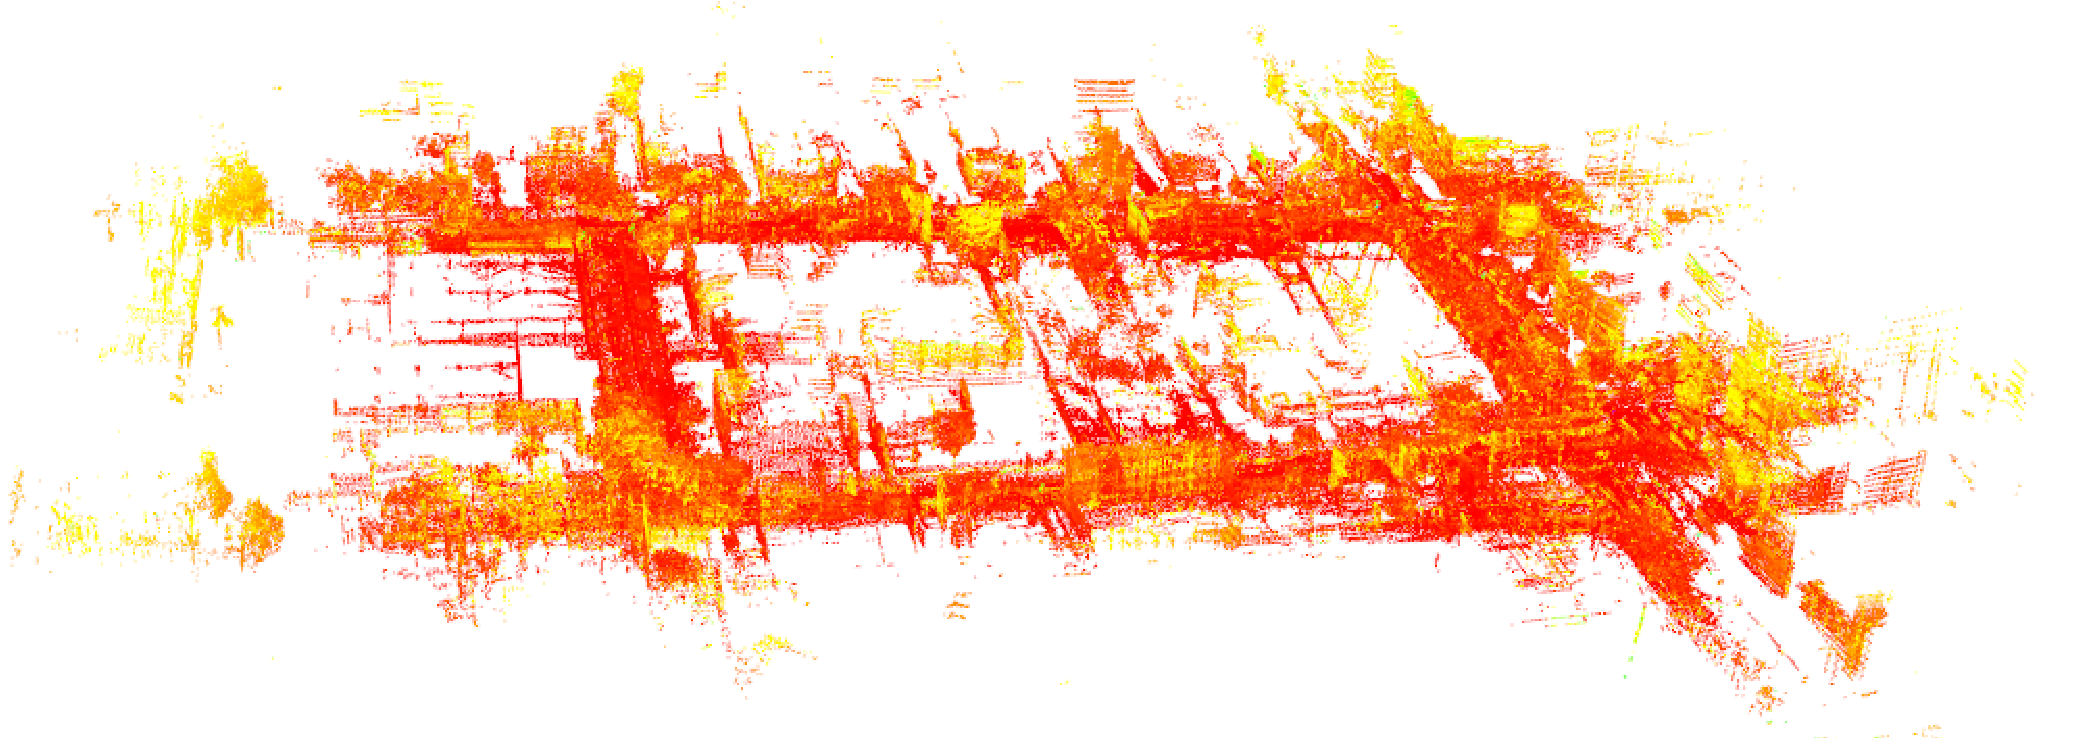
\includegraphics[width=1.0\textwidth]{resources/3d-lidar-mapping/ulhk-odom}
	\caption{Incremental NDT output (alternate view)}
	\label{fig:ulhk-odom}
\end{figure}

With visualization disabled, our incremental NDT processes each frame in ~6ms, compared to ~100ms for PCL's NDT - a >10× speedup. This demonstrates how understanding algorithmic principles enables custom optimizations beyond library limitations. Historical implementations often don't meet modern efficiency standards or anticipate future needs.

Both this and the next section present \textbf{pure LiDAR} odometry. While adequate for passenger vehicle datasets, they may struggle with rapidly rotating small vehicles. Later we'll enhance them with IMU and RTK measurements for robust performance.

\section{Laser Odometry with Feature-based Methods}  
\subsection{Feature Extraction}  

We refer to the odometry that \textbf{directly registers point clouds} as the direct method odometry. In contrast, autonomous driving often employs odometry that \textbf{first extracts features and then performs registration}, which we call feature-based odometry (or indirect method odometry) \cite{Wei2020}. Feature-based odometry requires extracting simple features from the point cloud first, followed by registering only the feature points. Additionally, depending on the different properties of the feature points themselves, different registration methods can be applied to achieve higher accuracy \cite{Hata2015}. Feature-based odometry implements different registration methods for different point cloud structures, offering better generalization compared to direct method odometry, which uniformly uses ICP or NDT. Among feature-based odometry systems, the LOAM series \cite{Zhang2014}, including the original LOAM \cite{Zhang2014} and subsequent improved versions (LeGO-LOAM \cite{Shan2018}, A-LOAM\footnote{\url{https://github.com/HKUST-Aerial-Robotics/A-LOAM}}, F-LOAM\footnote{\url{https://github.com/wh200720041/floam}}), are widely used open-source solutions in the autonomous driving industry and serve as the foundation for many subsequent LIO systems. However, the actual LOAM open-source code is quite complex, and we do not intend to explain it line by line in this book. Instead, we will explore the design philosophy of the LOAM series and provide a simple implementation based on its principles.  

When discussing feature-based methods, the most pressing questions are: For a multi-beam LiDAR, what kind of features should we extract? And how should we use these features for point cloud registration? There are many types of point cloud features, such as PFH \cite{Rusu2008}, FPFH \cite{Rusu2009a}, and various deep learning-based features. We must ask: What kind of features are meaningful for real-time registration? Point cloud features can be used not only for registration but also for database retrieval, comparison, and compression. In real-time SLAM, we have the following requirements for features:  
\begin{enumerate}  
	\item Features should reflect the characteristics of the point cloud. For example, point clouds in autonomous driving are typically scanned by multi-beam LiDARs and are not as dense as RGB-D point clouds. Instead, they exhibit distinct \textbf{beam} properties, where each point belongs to a specific beam of the LiDAR. Instead of extracting features directly from the entire point cloud, we can extract features from the scan data of individual beams.  
	\item After feature extraction, it should be straightforward to perform geometric registration on these feature points. Registration methods such as ICP or NDT can be used.  
	\item Feature extraction should not consume excessive CPU or GPU resources, nor should it require specialized hardware.  
	\item In system design, we prefer the entire LO or SLAM system to use the same computational architecture, rather than having some parts run on the CPU and others on the GPU, which would lead to unnecessary data transfer and resource consumption.  
\end{enumerate}  

Therefore, in industrial LO systems, people often use simple feature structures rather than complex ones based on statistical information or neural network computations. Most systems utilize \textbf{beam} information for feature extraction. Below, we introduce the feature extraction method used in LOAM-like systems.

\subsection{Feature Extraction Based on LiDAR Beams}  

Multi-beam LiDARs inherently provide \textbf{beam} information. In addition to the positional data $(x, y, z)$, the point cloud obtained from a LiDAR includes the following extra information:  
\begin{enumerate}  
	\item Which scan line a laser point originates from;  
	\item The sequential order of laser points on the same scan line;  
	\item Some drivers also output precise information such as polar coordinates and scan timestamps for each point.  
\end{enumerate}  

Knowing which points belong to the same scan line and their temporal order is highly useful for designing LiDAR odometry algorithms. Most notably, it eliminates the need to search for nearest neighbors on the same scan line. Additionally, based on the sequential order of these points, we can compute their \textbf{curvature} and classify them accordingly. The curvature can be defined as the difference between a point and its neighboring points on the same beam. In the LOAM series of work, researchers proposed a straightforward approach: points with high curvature along the same beam are classified as corner points, while those with low curvature are classified as planar points. To select the most distinct corner and planar points, one can sample the points with the highest and lowest curvature values, respectively. In multi-beam LiDAR scans, corner points typically lie on the surfaces of vertical objects or at the intersection of two planes, making them suitable for point-to-line ICP in the vertical direction. Meanwhile, planar points can be sampled across different beams and registered using point-to-plane ICP. The entire feature extraction and nearest-neighbor process is illustrated in Fig.~\ref{fig:curvature}.  

\begin{figure}[!thp]  
	\centering  
	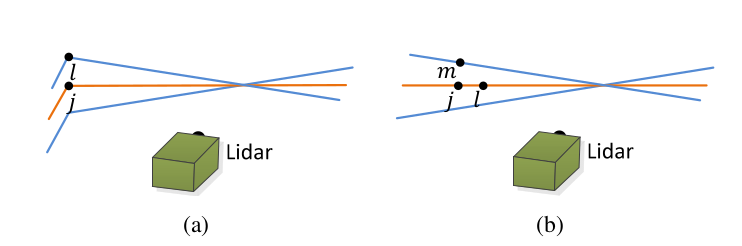
\includegraphics[width=.8\textwidth]{resources/3d-lidar-mapping/curvature.png}  
	\caption{Using beam curvature to identify corner and planar points, followed by nearest-neighbor matching. The left side shows points $l$ and $j$ forming a line, while the right side shows points $m$, $j$, and $l$ forming a plane. This figure is sourced from \cite{Zhang2014}.}  
	\label{fig:curvature}  
\end{figure}  

It is worth noting that this method of extracting corner and planar points can also be applied to 2D LiDARs, allowing the same approach to be used in 2D scan matching. Moreover, the extraction method is not limited to this single technique. For example, LeGO-LOAM \cite{Shan2018} uses range images to extract ground points, corner points, and planar points, while MULLS employs PCA to extract features such as ground, facades, pillars, and horizontal lines \cite{Pan2021}. However, most practical systems involve complex feature extraction processes, the details of which we will not cover here. Readers need only understand that extracting features to some extent helps optimize registration results.  

That said, this beam-based method relies heavily on prior knowledge, such as the assumption that the point cloud consists of multiple scan lines and that the LiDAR is horizontally mounted. These implementations are often highly engineering-dependent, tailored to specific LiDAR scan angles and beam configurations. Such assumptions do not hold for solid-state LiDARs or RGB-D camera point clouds, limiting the applicability of this odometry approach.  

\subsection{Implementation of Feature Extraction}  

We will now implement the feature extraction component. Beam-based feature extraction requires knowledge of the LiDAR's beam information, which some LiDAR drivers provide. However, if the point cloud is converted to a standard PCL format, this information may be lost. While it is possible to compute the elevation angle for each point and infer its beam based on the LiDAR's elevation angle specifications, this complicates the code and introduces additional dependencies, increasing the learning curve for this book. Instead, we provide readers with preprocessed point clouds that include beam information, allowing them to focus solely on computing corner and planar points.  

The feature extraction algorithm consists of the following steps:  
\begin{enumerate}  
	\item Compute and categorize each point's beam. Since our point clouds already include this information, this step can be skipped.  
	\item Sequentially compute the curvature for each point on a beam.  
	\item Divide the point cloud into sectors (we use six sectors in this implementation). Select points with the highest curvature as corner points, while the remaining points are classified as planar points.  
\end{enumerate}  

Note that most feature extraction methods lack rigorous theoretical justification and are instead derived from empirical engineering practices. Readers are encouraged to modify the feature extraction pipeline as needed, adding or removing steps as appropriate. Below is the code implementation:  

\begin{lstlisting}[language=c++,caption=src/ch7/loam\_like/feature\_extraction.cc]  
	void FeatureExtraction::Extract(FullCloudPtr pc_in, CloudPtr pc_out_edge, CloudPtr pc_out_surf) {  
		int num_scans = 16;  
		std::vector<CloudPtr> scans_in_each_line;  // Point clouds grouped by beam  
		for (int i = 0; i < num_scans; i++) {  
			scans_in_each_line.emplace_back(new PointCloudType);  
		}  
		
		for (auto &pt : pc_in->points) {  
			assert(pt.ring >= 0 && pt.ring < num_scans);  
			PointType p;  
			p.x = pt.x;  
			p.y = pt.y;  
			p.z = pt.z;  
			p.intensity = pt.intensity;  
			
			scans_in_each_line[pt.ring]->emplace_back(p);  
		}  
		
		// Compute curvature  
		for (int i = 0; i < num_scans; i++) {  
			if (scans_in_each_line[i]->points.size() < 131) {  
				continue;  
			}  
			
			std::vector<IdAndValue> cloud_curvature;  // Curvature for each beam  
			int total_points = scans_in_each_line[i]->points.size() - 10;  
			for (int j = 5; j < (int)scans_in_each_line[i]->points.size() - 5; j++) {  
				// Leave a margin at both ends, sampling 10 neighboring points for averaging  
				double diffX = scans_in_each_line[i]->points[j - 5].x + scans_in_each_line[i]->points[j - 4].x +  
				scans_in_each_line[i]->points[j - 3].x + scans_in_each_line[i]->points[j - 2].x +  
				scans_in_each_line[i]->points[j - 1].x - 10 * scans_in_each_line[i]->points[j].x +  
				scans_in_each_line[i]->points[j + 1].x + scans_in_each_line[i]->points[j + 2].x +  
				scans_in_each_line[i]->points[j + 3].x + scans_in_each_line[i]->points[j + 4].x +  
				scans_in_each_line[i]->points[j + 5].x;  
				double diffY = scans_in_each_line[i]->points[j - 5].y + scans_in_each_line[i]->points[j - 4].y +  
				scans_in_each_line[i]->points[j - 3].y + scans_in_each_line[i]->points[j - 2].y +  
				scans_in_each_line[i]->points[j - 1].y - 10 * scans_in_each_line[i]->points[j].y +  
				scans_in_each_line[i]->points[j + 1].y + scans_in_each_line[i]->points[j + 2].y +  
				scans_in_each_line[i]->points[j + 3].y + scans_in_each_line[i]->points[j + 4].y +  
				scans_in_each_line[i]->points[j + 5].y;  
				double diffZ = scans_in_each_line[i]->points[j - 5].z + scans_in_each_line[i]->points[j - 4].z +  
				scans_in_each_line[i]->points[j - 3].z + scans_in_each_line[i]->points[j - 2].z +  
				scans_in_each_line[i]->points[j - 1].z - 10 * scans_in_each_line[i]->points[j].z +  
				scans_in_each_line[i]->points[j + 1].z + scans_in_each_line[i]->points[j + 2].z +  
				scans_in_each_line[i]->points[j + 3].z + scans_in_each_line[i]->points[j + 4].z +  
				scans_in_each_line[i]->points[j + 5].z;  
				IdAndValue distance(j, diffX * diffX + diffY * diffY + diffZ * diffZ);  
				cloud_curvature.push_back(distance);  
			}  
			
			// Select features per sector (360° divided into 6 sectors)  
			for (int j = 0; j < 6; j++) {  
				int sector_length = (int)(total_points / 6);  
				int sector_start = sector_length * j;  
				int sector_end = sector_length * (j + 1) - 1;  
				if (j == 5) {  
					sector_end = total_points - 1;  
				}  
				
				std::vector<IdAndValue> sub_cloud_curvature(cloud_curvature.begin() + sector_start,  
				cloud_curvature.begin() + sector_end);  
				
				ExtractFromSector(scans_in_each_line[i], sub_cloud_curvature, pc_out_edge, pc_out_surf);  
			}  
		}  
	}  
	
	void FeatureExtraction::ExtractFromSector(const CloudPtr &pc_in, std::vector<IdAndValue> &cloud_curvature, CloudPtr &pc_out_edge, CloudPtr &pc_out_surf) {  
		// Sort by curvature  
		std::sort(cloud_curvature.begin(), cloud_curvature.end(),  
		[](const IdAndValue &a, const IdAndValue &b) { return a.value_ < b.value_; });  
		
		int largest_picked_num = 0;  
		int point_info_count = 0;  
		
		/// Select corner points with the highest curvature  
		std::vector<int> picked_points;  // Mark selected corner points (neighboring points are excluded)  
		for (int i = cloud_curvature.size() - 1; i >= 0; i--) {  
			int ind = cloud_curvature[i].id_;  
			if (std::find(picked_points.begin(), picked_points.end(), ind) == picked_points.end()) {  
				if (cloud_curvature[i].value_ <= 0.1) {  
					break;  
				}  
				
				largest_picked_num++;  
				picked_points.push_back(ind);  
				
				if (largest_picked_num <= 20) {  
					pc_out_edge->push_back(pc_in->points[ind]);  
					point_info_count++;  
				} else {  
					break;  
				}  
				
				for (int k = 1; k <= 5; k++) {  
					double diffX = pc_in->points[ind + k].x - pc_in->points[ind + k - 1].x;  
					double diffY = pc_in->points[ind + k].y - pc_in->points[ind + k - 1].y;  
					double diffZ = pc_in->points[ind + k].z - pc_in->points[ind + k - 1].z;  
					if (diffX * diffX + diffY * diffY + diffZ * diffZ > 0.05) {  
						break;  
					}  
					picked_points.push_back(ind + k);  
				}  
				for (int k = -1; k >= -5; k--) {  
					double diffX = pc_in->points[ind + k].x - pc_in->points[ind + k + 1].x;  
					double diffY = pc_in->points[ind + k].y - pc_in->points[ind + k + 1].y;  
					double diffZ = pc_in->points[ind + k].z - pc_in->points[ind + k + 1].z;  
					if (diffX * diffX + diffY * diffY + diffZ * diffZ > 0.05) {  
						break;  
					}  
					picked_points.push_back(ind + k);  
				}  
			}  
		}  
		
		/// Select planar points with lower curvature  
		for (int i = 0; i <= (int)cloud_curvature.size() - 1; i++) {  
			int ind = cloud_curvature[i].id_;  
			if (std::find(picked_points.begin(), picked_points.end(), ind) == picked_points.end()) {  
				pc_out_surf->push_back(pc_in->points[ind]);  
			}  
		}  
	}  
\end{lstlisting}  

The entire process aligns with the description above. We use the `test_feature_extraction` program to evaluate the extraction results on a single point cloud. The program reads raw Velodyne packets and converts them into a point cloud while preserving beam information. The feature extraction algorithm then separates corner and planar points, storing them in two PCD files, as shown in Fig.~\ref{fig:corner-and-edge}. In structured indoor environments, corner and planar points are clearly distinguishable—corners lie on edges, while planar points lie on surfaces. In outdoor open areas, planar points perform well, but corner points are less reliable. Additionally, ground points are often distributed in circular patterns rather than straight lines, making curvature-based classification less effective. Some odometry algorithms opt to filter out ground points or model them separately. Similar approaches are used for ceilings in indoor environments.  

\begin{figure}[!thp]  
	\centering  
	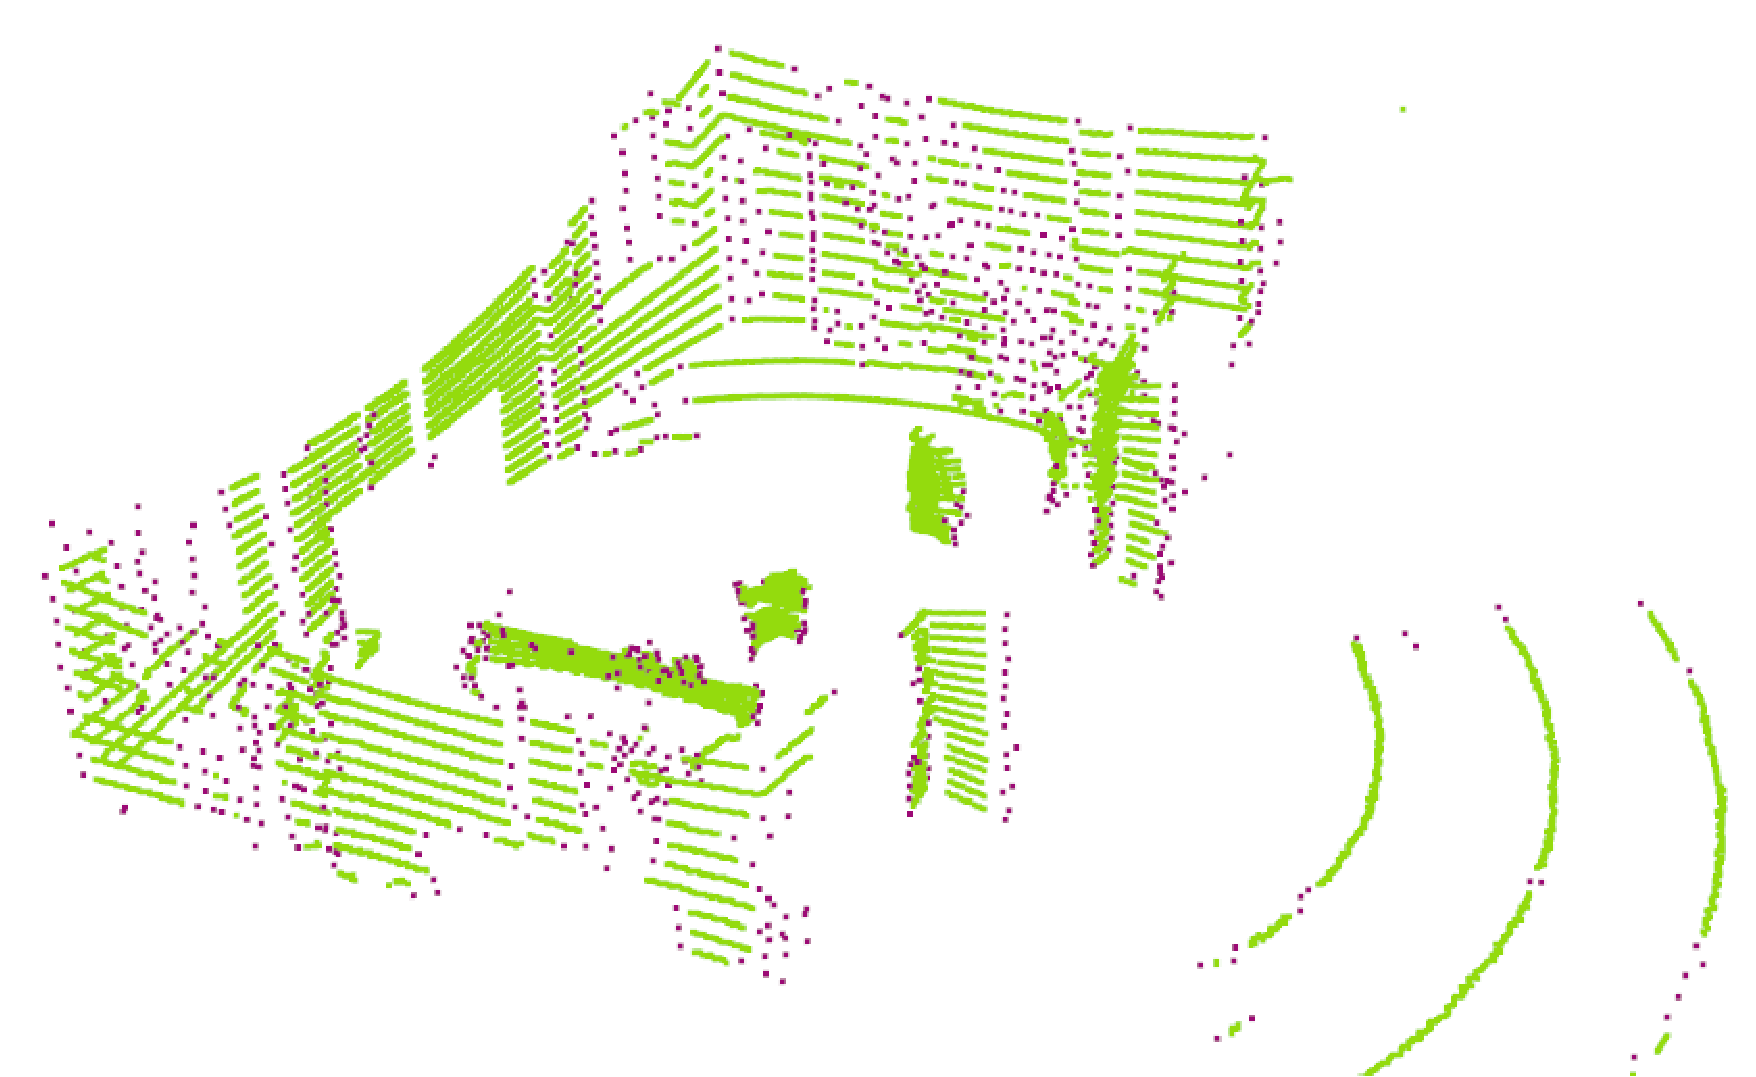
\includegraphics[width=.8\textwidth]{resources/3d-lidar-mapping/corner_and_edge}  
	\caption{Corner and planar points extracted from a single scan. Red points: corners (or edges); green points: planar points.}  
	\label{fig:corner-and-edge}  
\end{figure}  

\begin{figure}[!thp]  
	\centering  
	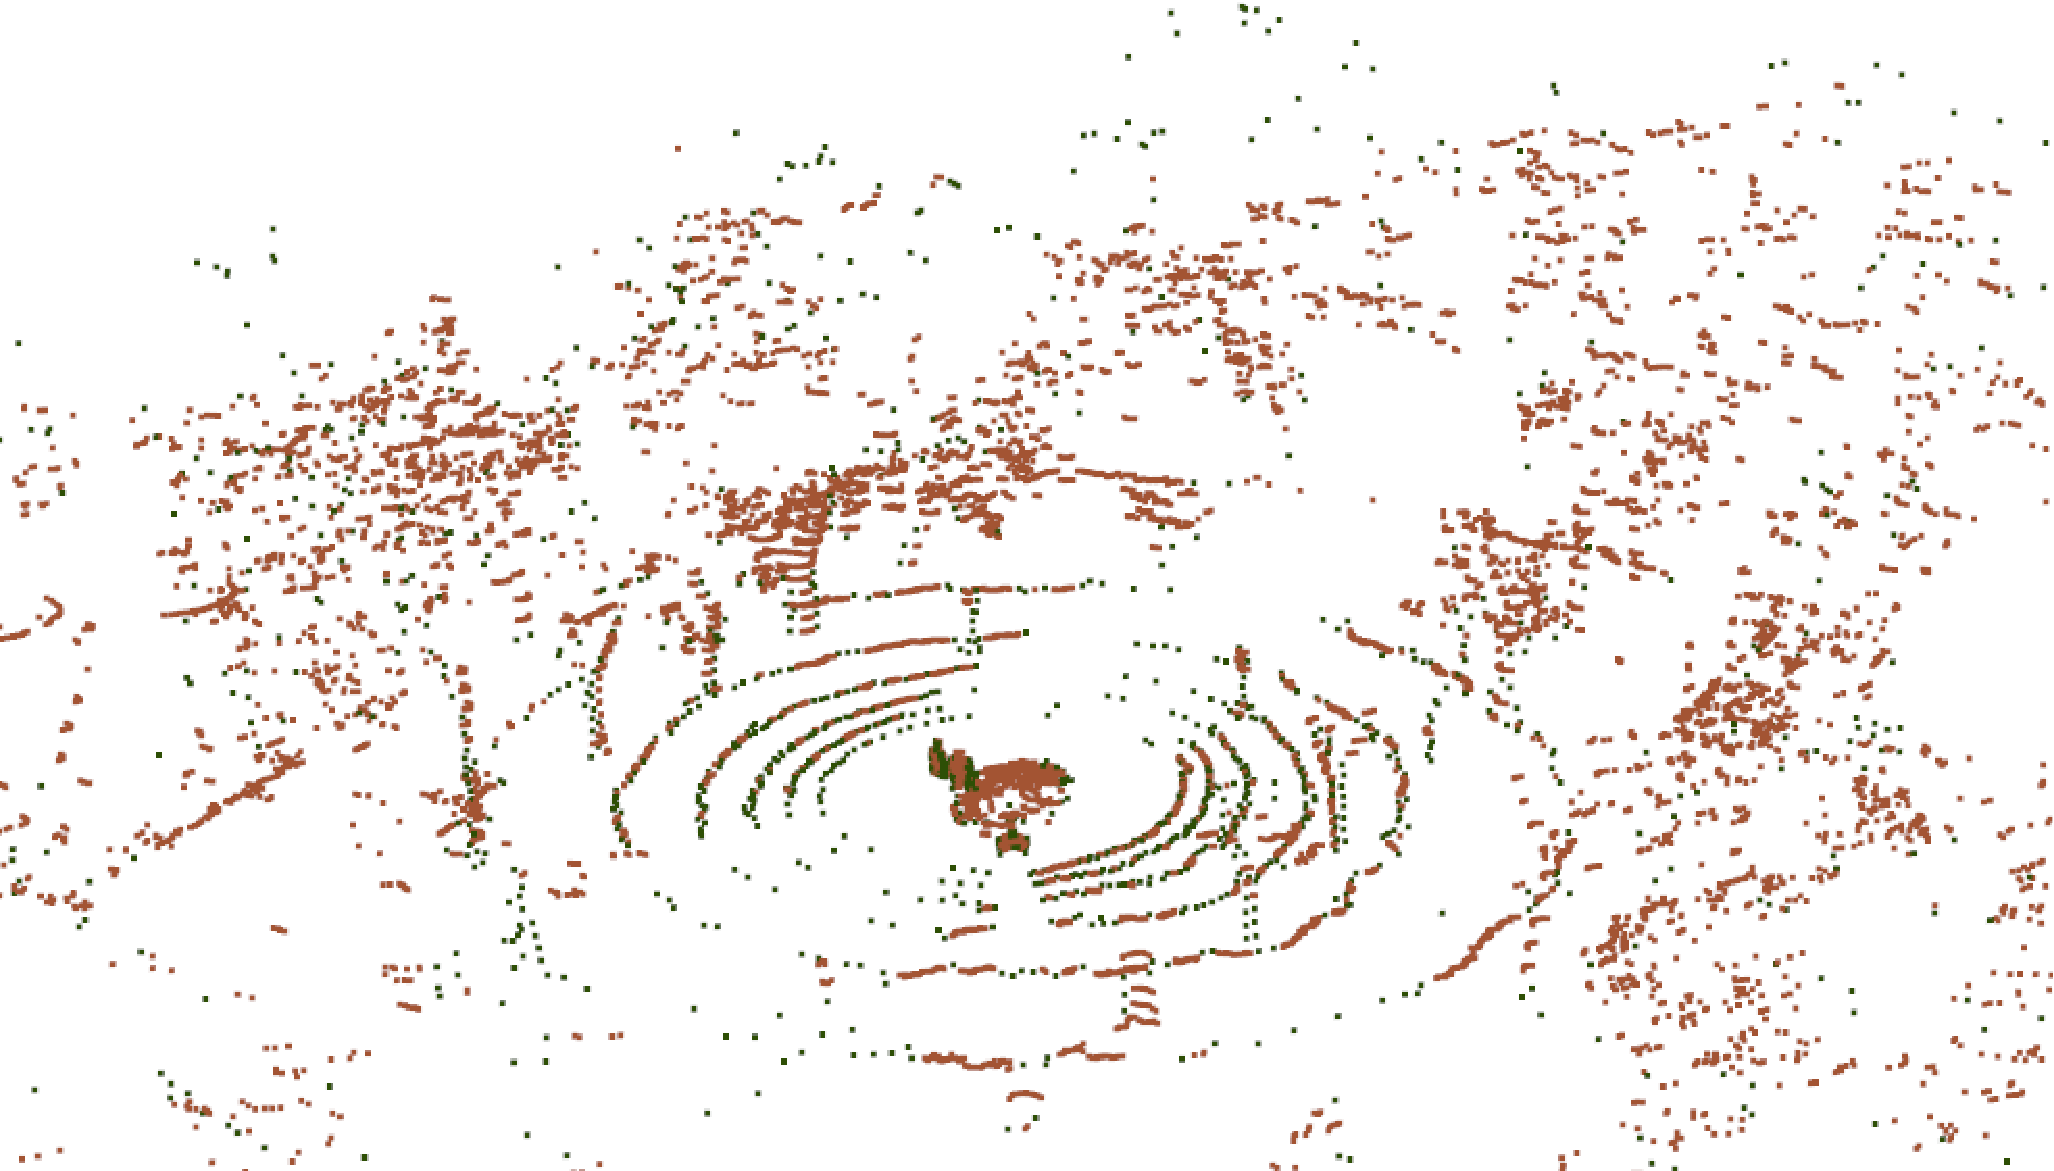
\includegraphics[width=.8\textwidth]{resources/3d-lidar-mapping/corner-and-edge-outside}  
	\caption{Corner and planar points in an outdoor scene. Planar points: reddish-brown; corner points: green.}  
	\label{fig:corner-and-edge-outside}  
\end{figure}  

Feature extraction typically consumes significant computational resources, making feature-based odometry slower than direct registration methods. However, the results are often more stable.

Now let's implement the feature-based LiDAR odometry. The overall computational flow is similar to the previous NDT-based approach. We construct two local maps for corner and planar points respectively, then incorporate both ICP results into a single optimization problem. The core registration code is as follows:

\begin{lstlisting}[language=c++,caption=src/ch7/loam-like/loam\_like\_odom.cc]
	class LoamLikeOdom {
		public:
		struct Options {
			Options() {}
			
			int min_edge_pts_ = 20;               // Minimum edge points
			int min_surf_pts_ = 20;               // Minimum planar points
			double kf_distance_ = 1.0;            // Keyframe distance threshold
			double kf_angle_deg_ = 15;            // Rotation angle threshold
			int num_kfs_in_local_map_ = 30;       // Number of keyframes in local map
			bool display_realtime_cloud_ = true;  // Whether to display real-time cloud
			
			// ICP parameters
			int max_iteration_ = 5;             // Maximum iterations
			double max_plane_distance_ = 0.05;  // Plane distance threshold
			double max_line_distance_ = 0.5;    // Line distance threshold
			int min_effective_pts_ = 10;        // Minimum effective points
			double eps_ = 1e-3;                 // Convergence threshold
			
			bool use_edge_points_ = true;  // Whether to use edge points
			bool use_surf_points_ = true;  // Whether to use planar points
		};
		
		explicit LoamLikeOdom(Options options = Options());
		
		/**
		* Process a point cloud, which will be divided into edge and planar points
		* @param pcd_edge
		* @param pcd_surf
		*/
		void ProcessPointCloud(FullCloudPtr full_cloud);
		
		private:
		/// Align with local map
		SE3 AlignWithLocalMap(CloudPtr edge, CloudPtr surf);
		
		/// Determine if current frame is keyframe
		bool IsKeyframe(const SE3& current_pose);
		
		Options options_;
		
		int cnt_frame_ = 0;
		int last_kf_id_ = 0;
		
		CloudPtr local_map_edge_ = nullptr, local_map_surf_ = nullptr;  // Local maps
		std::vector<SE3> estimated_poses_;    // Estimated poses for trajectory
		SE3 last_kf_pose_;                    // Last keyframe pose
		std::deque<CloudPtr> edges_, surfs_;  // Cached edge and planar points
		
		CloudPtr global_map_ = nullptr;  // Global map for saving
		
		std::shared_ptr<FeatureExtraction> feature_extraction_ = nullptr;
		
		std::shared_ptr<PCLMapViewer> viewer_ = nullptr;
		KdTree kdtree_edge_, kdtree_surf_;
	};
	
	void LoamLikeOdom::ProcessPointCloud(FullCloudPtr cloud) {
		LOG(INFO) << "processing frame " << cnt_frame_++;
		// Step 1. Feature extraction
		CloudPtr current_edge(new PointCloudType), current_surf(new PointCloudType);
		feature_extraction_->Extract(cloud, current_edge, current_surf);
		
		if (current_edge->size() < options_.min_edge_pts_ || current_surf->size() < options_.min_surf_pts_) {
			LOG(ERROR) << "not enough edge/surf pts: " << current_edge->size() << "," << current_surf->size();
			return;
		}
		
		LOG(INFO) << "edge: " << current_edge->size() << ", surf: " << current_surf->size();
		
		if (local_map_edge_ == nullptr || local_map_surf_ == nullptr) {
			// Special handling for first frame
			local_map_edge_ = current_edge;
			local_map_surf_ = current_surf;
			
			kdtree_edge_.BuildTree(local_map_edge_);
			kdtree_surf_.BuildTree(local_map_surf_);
			
			edges_.emplace_back(current_edge);
			surfs_.emplace_back(current_surf);
			return;
		}
		
		/// Align with local map
		SE3 pose = AlignWithLocalMap(current_edge, current_surf);
		CloudPtr scan_world(new PointCloudType);
		pcl::transformPointCloud(*ConvertToCloud<FullPointType>(cloud), *scan_world, pose.matrix());
		
		CloudPtr edge_world(new PointCloudType), surf_world(new PointCloudType);
		pcl::transformPointCloud(*current_edge, *edge_world, pose.matrix());
		pcl::transformPointCloud(*current_surf, *surf_world, pose.matrix());
		
		if (IsKeyframe(pose)) {
			LOG(INFO) << "inserting keyframe";
			last_kf_pose_ = pose;
			last_kf_id_ = cnt_frame_;
			
			// Rebuild local map
			edges_.emplace_back(edge_world);
			surfs_.emplace_back(surf_world);
			
			if (edges_.size() > options_.num_kfs_in_local_map_) {
				edges_.pop_front();
			}
			if (surfs_.size() > options_.num_kfs_in_local_map_) {
				surfs_.pop_front();
			}
			
			local_map_surf_.reset(new PointCloudType);
			local_map_edge_.reset(new PointCloudType);
			
			for (auto& s : edges_) {
				*local_map_edge_ += *s;
			}
			for (auto& s : surfs_) {
				*local_map_surf_ += *s;
			}
			
			local_map_surf_ = VoxelCloud(local_map_surf_, 1.0);
			local_map_edge_ = VoxelCloud(local_map_edge_, 1.0);
			
			LOG(INFO) << "insert keyframe, surf pts: " << local_map_surf_->size()
			<< ", edge pts: " << local_map_edge_->size();
			
			kdtree_surf_.BuildTree(local_map_surf_);
			kdtree_edge_.BuildTree(local_map_edge_);
			
			*global_map_ += *scan_world;
		}
		
		LOG(INFO) << "current pose: " << pose.translation().transpose() << ", "
		<< pose.so3().unit_quaternion().coeffs().transpose();
		
		if (viewer_ != nullptr) {
			viewer_->SetPoseAndCloud(pose, scan_world);
		}
	}
	
	SE3 LoamLikeOdom::AlignWithLocalMap(CloudPtr edge, CloudPtr surf) {
		// Custom ICP implementation needed here
		SE3 pose;
		if (estimated_poses_.size() >= 2) {
			// Predict pose from last two poses
			SE3 T1 = estimated_poses_[estimated_poses_.size() - 1];
			SE3 T2 = estimated_poses_[estimated_poses_.size() - 2];
			pose = T1 * (T2.inverse() * T1);
		}
		
		int edge_size = edge->size();
		int surf_size = surf->size();
		
		// Implement concurrent processing
		for (int iter = 0; iter < options_.max_iteration_; ++iter) {
			std::vector<bool> effect_surf(surf_size, false);
			std::vector<Eigen::Matrix<double, 1, 6>> jacob_surf(surf_size);  // 1D residual for planes
			std::vector<double> errors_surf(surf_size);
			
			std::vector<bool> effect_edge(edge_size, false);
			std::vector<Eigen::Matrix<double, 3, 6>> jacob_edge(edge_size);  // 3D residual for edges
			std::vector<Vec3d> errors_edge(edge_size);
			
			std::vector<int> index_surf(surf_size);
			std::iota(index_surf.begin(), index_surf.end(), 0);
			std::vector<int> index_edge(edge_size);
			std::iota(index_edge.begin(), index_edge.end(), 0);
			
			// Gauss-Newton iteration
			// Nearest neighbor search for edge points
			if (options_.use_edge_points_) {
				std::for_each(std::execution::par_unseq, index_edge.begin(), index_edge.end(), [&](int idx) {
					Vec3d q = ToVec3d(edge->points[idx]);
					Vec3d qs = pose * q;
					
					// Find nearest neighbors
					std::vector<int> nn_indices;
					
					kdtree_edge_.GetClosestPoint(ToPointType(qs), nn_indices, 5);
					effect_edge[idx] = false;
					
					if (nn_indices.size() >= 3) {
						std::vector<Vec3d> nn_eigen;
						for (auto& n : nn_indices) {
							nn_eigen.emplace_back(ToVec3d(local_map_edge_->points[n]));
						}
						
						// Point-to-line residual
						Vec3d d, p0;
						if (!math::FitLine(nn_eigen, p0, d, options_.max_line_distance_)) {
							return;
						}
						
						Vec3d err = SO3::hat(d) * (qs - p0);
						if (err.norm() > options_.max_line_distance_) {
							return;
						}
						
						effect_edge[idx] = true;
						
						// Build residual
						Eigen::Matrix<double, 3, 6> J;
						J.block<3, 3>(0, 0) = -SO3::hat(d) * pose.so3().matrix() * SO3::hat(q);
						J.block<3, 3>(0, 3) = SO3::hat(d);
						
						jacob_edge[idx] = J;
						errors_edge[idx] = err;
					}
				});
			}
			
			/// Nearest neighbor search for planar points
			if (options_.use_surf_points_) {
				std::for_each(std::execution::par_unseq, index_surf.begin(), index_surf.end(), [&](int idx) {
					Vec3d q = ToVec3d(surf->points[idx]);
					Vec3d qs = pose * q;
					
					// Find nearest neighbors
					std::vector<int> nn_indices;
					
					kdtree_surf_.GetClosestPoint(ToPointType(qs), nn_indices, 5);
					effect_surf[idx] = false;
					
					if (nn_indices.size() == 5) {
						std::vector<Vec3d> nn_eigen;
						for (auto& n : nn_indices) {
							nn_eigen.emplace_back(ToVec3d(local_map_surf_->points[n]));
						}
						
						// Point-to-plane residual
						Vec4d n;
						if (!math::FitPlane(nn_eigen, n)) {
							return;
						}
						
						double dis = n.head<3>().dot(qs) + n[3];
						if (fabs(dis) > options_.max_plane_distance_) {
							return;
						}
						
						effect_surf[idx] = true;
						
						// Build residual
						Eigen::Matrix<double, 1, 6> J;
						J.block<1, 3>(0, 0) = -n.head<3>().transpose() * pose.so3().matrix() * SO3::hat(q);
						J.block<1, 3>(0, 3) = n.head<3>().transpose();
						
						jacob_surf[idx] = J;
						errors_surf[idx] = dis;
					}
				});
			}
			
			// Accumulate Hessian and error, compute dx
			double total_res = 0;
			int effective_num = 0;
			
			Mat6d H = Mat6d::Zero();
			Vec6d err = Vec6d::Zero();
			
			for (const auto& idx : index_surf) {
				if (effect_surf[idx]) {
					H += jacob_surf[idx].transpose() * jacob_surf[idx];
					err += -jacob_surf[idx].transpose() * errors_surf[idx];
					effective_num++;
					total_res += errors_surf[idx] * errors_surf[idx];
				}
			}
			
			for (const auto& idx : index_edge) {
				if (effect_edge[idx]) {
					H += jacob_edge[idx].transpose() * jacob_edge[idx];
					err += -jacob_edge[idx].transpose() * errors_edge[idx];
					effective_num++;
					total_res += errors_edge[idx].norm();
				}
			}
			
			if (effective_num < options_.min_effective_pts_) {
				LOG(WARNING) << "effective num too small: " << effective_num;
				return pose;
			}
			
			Vec6d dx = H.inverse() * err;
			pose.so3() = pose.so3() * SO3::exp(dx.head<3>());
			pose.translation() += dx.tail<3>();
			
			// Update
			LOG(INFO) << "iter " << iter << " total res: " << total_res << ", eff: " << effective_num
			<< ", mean res: " << total_res / effective_num << ", dxn: " << dx.norm();
			
			if (dx.norm() < options_.eps_) {
				LOG(INFO) << "converged, dx = " << dx.transpose();
				break;
			}
		}
		
		estimated_poses_.emplace_back(pose);
		return pose;
	}
\end{lstlisting}

Since we need to handle both point-to-line and point-to-plane registration simultaneously, the code here will be somewhat lengthy. The workflow is identical to what we introduced in the ICP section, with the addition of local map maintenance procedures. Readers should compile and run the `test_loam_odom` program to execute this odometry:

\begin{lstlisting}[language=c++,caption=Terminal input:]
	bin/test_loam_odom 
\end{lstlisting}

Figure~\ref{fig:loam-map} shows the mapping results from this section's odometry program, where readers can clearly observe the structural shapes of various objects.

\begin{figure}[!thp]
	\centering  
	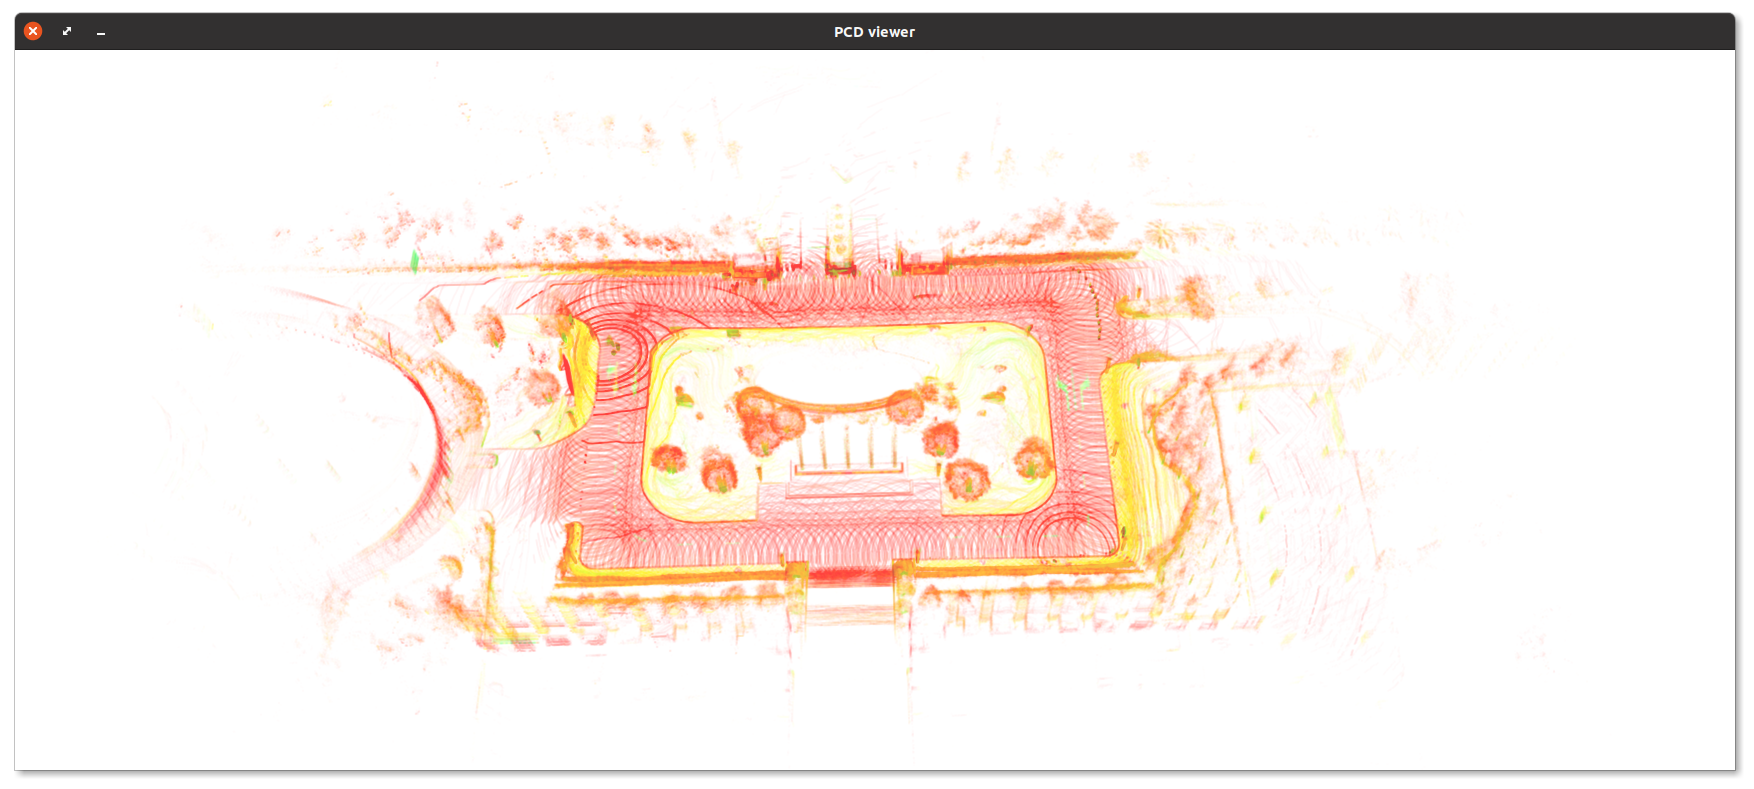
\includegraphics[width=.8\textwidth]{resources/3d-lidar-mapping/ch7-loam-map}  
	\caption{Point cloud map generated by the LOAM-like odometry algorithm in this section}  
	\label{fig:loam-map}  
\end{figure}

In principle, feature-based algorithms classify raw point clouds into simple features and then construct different optimization problems for different feature types. The rationale behind extracting these features and using different ICP methods for corner and planar points remains largely based on empirical debugging experience. In practical testing, corner and planar points cannot always be perfectly classified—they represent approximate results. Many points classified as corners or planes may actually lie on trees or bushes, where point-to-plane ICP might not reflect true physical meaning. Therefore, feature-based point cloud registration methods are primarily designed based on intuitive experience. They may perform better on certain datasets but fail in other scenarios. Many feature extraction processes also lack theoretical foundations, relying instead on empirical design. Systems like LeGO-LOAM and MULLS employ more sophisticated feature extraction methods, while their registration components remain consistent with classical algorithms.  

We can further refine the classification by separating ground and ceiling points, categorizing point clouds into \textbf{corners, less-sharp corners, planar points, less-flat planar points}, etc., based on beam curvature. Such refinements can improve registration accuracy.  

In terms of performance metrics, this odometry processes 16-beam LiDAR data at approximately 20 milliseconds per frame, slightly slower than the incremental NDT odometry discussed earlier. This is partly due to the added feature extraction step and the need to rebuild Kd-trees for nearest-neighbor searches in point-to-plane and point-to-line ICP. Some methods use voxels for ICP nearest-neighbor searches instead—readers are encouraged to implement this themselves.  

In addition to the examples demonstrated in the book, readers can also run other provided sample datasets.

\section{Loosely Coupled LIO Systems}
By the previous section, we have systematically introduced LiDAR SLAM systems along with the principles of inertial navigation and integrated navigation. Now it's time to combine them together.

Many LiDAR odometry algorithms utilize IMU measurements to guide the initial guess for LiDAR matching. Such Lidar-inertial Odometry systems are referred to as LIO or LINS systems, which can be viewed as coupled LiDAR-IMU systems. Based on the coupling methodology, they can be classified into "tightly coupled" and "loosely coupled" systems. This section focuses on loosely coupled systems, while the theoretically more complex tightly coupled systems will be introduced in Chapter~\ref{cpt:tightly-lio}.

In a loosely coupled system, we still maintain a state estimator to compute the vehicle's state. The IMU and wheel odometry provide observations for inertial and velocity states, while \textbf{the pose output from LiDAR point cloud matching} serves as pose observations for the system. In this framework, we do not directly incorporate point cloud residuals (such as point-to-line, point-to-plane, or NDT residuals) into the state estimator. Instead, we fuse the \textbf{output pose} from point cloud registration with the estimator. This keeps the Kalman filter component and point cloud registration \textbf{decoupled} \cite{Tang2015}. We can freely choose any odometry pose from previous chapters as the observation source. Conversely, point cloud registration can use the predicted output from the state estimator as the initial pose guess. However, if the point cloud structure degenerates or gets disturbed, the registration algorithm may become unstable, adversely affecting the state estimator.

In contrast, tightly coupled systems directly incorporate point cloud residual equations as observation models into the estimator. This approach essentially embeds an ICP or NDT process within the filter or optimization algorithm. Since ICP and NDT require iterative updates of their nearest neighbors, the corresponding filter should also support iterative updates. Having introduced various registration methods in this chapter and different inertial navigation approaches in earlier chapters, we can flexibly combine them to create an LIO solution. Here we implement a relatively simple case: using the ESKF from Chapter 3 combined with the incremental NDT odometry from Section \ref{sec:inc-ndt} to build a loosely coupled LIO system. This implementation is relatively simple and suitable for teaching purposes, and readers can replace the LiDAR odometry with ICP or feature-based methods.

\subsection{Coordinate Frame Conventions}
With the introduction of IMU, we now have three coordinate frames: world frame (W), IMU frame (I), and LiDAR frame (L). The IMU and LiDAR frames are not coincident, with a transformation between them denoted as $\mathbf{T}_{IL}$. This parameter varies across different datasets depending on sensor mounting. We record $\mathbf{T}_{IL}$ for each dataset in configuration files and load it during program initialization.

For point cloud registration, several approaches exist. Since IMU motion models are derived in the IMU frame, we prefer to keep them unchanged without introducing additional variables. Therefore, we choose to transform LiDAR point clouds to the IMU frame using the extrinsic calibration. This makes the IMU frame the central reference for localization and mapping. The local maps in our LiDAR odometry are also maintained in the IMU frame. The transformation is straightforward: for a point $\mathbf{p}_L$ measured by the LiDAR, its IMU frame coordinates become:
\begin{equation}\label{key}
	\mathbf{p}_{I} = \mathbf{T}_{IL} \mathbf{p}_L = \mathbf{R}_{IL} \mathbf{p}_L + \mathbf{t}_{IL}.
\end{equation}

This approach avoids introducing additional extrinsic parameters into the observation model. An alternative method would keep the LiDAR odometry operating in the LiDAR frame while transforming the output pose to the IMU frame via $\mathbf{T}_{IL}$. However, that would introduce extra $\mathbf{T}_{IL}$ terms in the observation equations, complicating the Jacobian matrices.

\subsection{Motion and Observation Equations for Loosely Coupled LIO}
Since the entire LIO operates in the IMU frame, the state variable motion equations remain consistent with~\eqref{eq:eskf-F}, which we won't reiterate here. Meanwhile, the pose output from LiDAR odometry can be directly treated as observations of the state variables $\mathbf{R}, \mathbf{p}$. This process is essentially identical to the GNSS observations discussed in Chapter~\ref{cpt:ins} equation~\eqref{eq:obs-gnss}. Abstractly written as $\mathbf{z}=\mathbf{h}(\mathbf{x})$, the translation observation is:
\begin{equation}\label{key}
	\mathbf{p}_{LO} = \mathbf{p}.
\end{equation}
For rotation observations, to facilitate derivative computation, we express it as:
\begin{equation}\label{key}
	\delta \boldsymbol{\theta} = \mathrm{Log}(\mathbf{R}^\top \mathbf{R}_{LO}).
\end{equation}
Here, the observation Jacobian of odometry rotation with respect to error state $\delta \boldsymbol{\theta}$ should be $\mathbf{I}$, with the residual defined as:
\begin{equation}\label{key}
	\mathbf{r}_{\mathbf{R}} = - \mathrm{Log}( \mathbf{R}^\top \mathbf{R}_{LO}).
\end{equation}
At the implementation level, we'll use the same observation function as GNSS since they fundamentally represent direct observations of rotation and translation.

\subsection{Data Preparation for Loosely Coupled System}
The implementation of loosely coupled LIO consists of three main components: First, we need to synchronize IMU data with LiDAR data. LiDAR typically operates at 10Hz while IMU runs at 100Hz. We aim to uniformly process the 10 IMU measurements between consecutive LiDAR scans. Second, we need to handle LiDAR motion compensation, which requires pose estimates during the LiDAR measurement period - these can be obtained from ESKF predictions of IMU data. Third, we should feed the predicted poses from ESKF to the odometry algorithm, then incorporate the registered poses back into ESKF. Additionally, to support various datasets in this book, we define an extra data conversion processor.

The CloudConvert class in this section handles conversion of different point cloud formats to PCL format, with the following main interface:

\begin{lstlisting}[language=c++,caption=src/ch7/loosly_coupled_lio/cloud_convert.h]
	class CloudConvert {
		public:
		EIGEN_MAKE_ALIGNED_OPERATOR_NEW
		
		enum class LidarType {
			AVIA = 1,  // DJI solid-state LiDAR
			VELO32,    // Velodyne 32-beam
			OUST64,    // Ouster 64-beam
		};
		
		CloudConvert() = default;
		~CloudConvert() = default;
		
		/**
		* Process Livox Avia point cloud
		* @param msg
		* @param pcl_out
		*/
		void Process(const livox_ros_driver::CustomMsg::ConstPtr &msg, FullCloudPtr &pcl_out);
		
		/**
		* Process sensor_msgs::PointCloud2
		* @param msg
		* @param pcl_out
		*/
		void Process(const sensor_msgs::PointCloud2::ConstPtr &msg, FullCloudPtr &pcl_out);
		
		/// Load parameters from YAML
		void LoadFromYAML(const std::string &yaml);
		
		private:
		void AviaHandler(const livox_ros_driver::CustomMsg::ConstPtr &msg);
		void Oust64Handler(const sensor_msgs::PointCloud2::ConstPtr &msg);
		void VelodyneHandler(const sensor_msgs::PointCloud2::ConstPtr &msg);
		
		FullPointCloudType cloud_full_, cloud_out_;  // Output point cloud
		LidarType lidar_type_ = LidarType::AVIA;     // LiDAR type
		int point_filter_num_ = 1;                   // Point decimation ratio
		int num_scans_ = 6;                          // Number of scan beams
		float time_scale_ = 1e-3;                    // Time field scaling factor
	};
\end{lstlisting}

The implementation mainly standardizes point cloud interfaces. After processing by this class, subsequent modules only need to handle FullCloudPtr input. The class manages per-point timestamps, decimation ratios, etc., typically producing much smaller point clouds than raw sensor output. We omit the detailed implementation as it's relatively trivial.

Next, we synchronize IMU and point cloud data using the MessageSync class:

\begin{lstlisting}[language=c++,caption=src/ch7/loosly_coupled_lio/measure_sync.h]
	/// IMU and LiDAR synchronization
	struct MeasureGroup {
		MeasureGroup() { this->lidar_.reset(new FullPointCloudType()); };
		
		double lidar_begin_time_ = 0;   // LiDAR packet start time
		double lidar_end_time_ = 0;     // LiDAR packet end time
		FullCloudPtr lidar_ = nullptr;  // LiDAR point cloud
		std::deque<IMUPtr> imu_;        // IMU measurements between frames
	};
	
	/**
	* Synchronize LiDAR and IMU data
	*/
	class MessageSync {
		public:
		using Callback = std::function<void(const MeasureGroup &)>;
		
		MessageSync(Callback cb) : callback_(cb), conv_(new CloudConvert) {}
		
		/// Initialization
		void Init(const std::string &yaml);
		
		/// Process IMU data
		void ProcessIMU(IMUPtr imu);
		
		/**
		* Process sensor_msgs::PointCloud2
		* @param msg
		*/
		void ProcessCloud(const sensor_msgs::PointCloud2::ConstPtr &msg);
		
		void ProcessCloud(const livox_ros_driver::CustomMsg::ConstPtr &msg);
		
		private:
		/// Attempt synchronization, returns true if successful
		bool Sync();
		
		Callback callback_;                             // Callback after synchronization
		std::shared_ptr<CloudConvert> conv_ = nullptr;  // Point cloud converter
		std::deque<FullCloudPtr> lidar_buffer_;         // LiDAR data buffer
		std::deque<IMUPtr> imu_buffer_;                 // IMU data buffer
		double last_timestamp_imu_ = -1.0;              // Latest IMU timestamp
		double last_timestamp_lidar_ = 0;               // Latest LiDAR timestamp
		std::deque<double> time_buffer_;
		bool lidar_pushed_ = false;
		MeasureGroup measures_;
		double lidar_end_time_ = 0;
	};
	
	bool MessageSync::Sync() {
		if (lidar_buffer_.empty() || imu_buffer_.empty()) {
			return false;
		}
		
		if (!lidar_pushed_) {
			measures_.lidar_ = lidar_buffer_.front();
			measures_.lidar_begin_time_ = time_buffer_.front();
			
			lidar_end_time_ = measures_.lidar_begin_time_ + 
			measures_.lidar_->points.back().time / double(1000);
			
			measures_.lidar_end_time_ = lidar_end_time_;
			lidar_pushed_ = true;
		}
		
		if (last_timestamp_imu_ < lidar_end_time_) {
			return false;
		}
		
		double imu_time = imu_buffer_.front()->timestamp_;
		measures_.imu_.clear();
		while ((!imu_buffer_.empty()) && (imu_time < lidar_end_time_)) {
			imu_time = imu_buffer_.front()->timestamp_;
			if (imu_time > lidar_end_time_) {
				break;
			}
			measures_.imu_.push_back(imu_buffer_.front());
			imu_buffer_.pop_front();
		}
		
		lidar_buffer_.pop_front();
		time_buffer_.pop_front();
		lidar_pushed_ = false;
		
		if (callback_) {
			callback_(measures_);
		}
		
		return true;
	}
\end{lstlisting}

This class receives raw IMU and LiDAR messages from ROS packages, assembles them into a MeasureGroup through the Sync() function, and passes it to the callback function. Our subsequent loosely/tightly coupled algorithms only need to handle MeasureGroup objects without worrying about data preparation and synchronization implementation details.

\subsection{Main Workflow of Loosely Coupled System}
The main implementation of the loosely coupled system is shown below. It maintains an ESKF object and a MessageSync object to process synchronized point clouds and IMU data.

\begin{lstlisting}[language=c++,caption=src/ch7/loosely_coupled_lio/loosly_lio.h]
	class LooselyLIO {
		public:
		EIGEN_MAKE_ALIGNED_OPERATOR_NEW;
		struct Options {
			Options() {}
			bool save_motion_undistortion_pcd_ = false;  // Whether to save point clouds before/after motion undistortion
			bool with_ui_ = true;                        // Whether to enable UI
		};
		
		LooselyLIO(Options options);
		~LooselyLIO() = default;
		
		/// Initialize from config file
		bool Init(const std::string &config_yaml);
		
		/// Point cloud callback
		void PCLCallBack(const sensor_msgs::PointCloud2::ConstPtr &msg);
		void LivoxPCLCallBack(const livox_ros_driver::CustomMsg::ConstPtr &msg);
		
		/// IMU callback
		void IMUCallBack(IMUPtr msg_in);
		
		/// Terminate program and exit UI
		void Finish();
		
		private:
		/// Process synchronized IMU and LiDAR data
		void ProcessMeasurements(const MeasureGroup &meas);
		
		/// Attempt IMU initialization
		void TryInitIMU();
		
		/// Predict states using IMU
		/// Predicted states during this period will be stored in imu_states_
		void Predict();
		
		/// Motion undistortion for point cloud in measures_
		void Undistort();
		
		/// Perform registration and observation
		void Align();
		
		private:
		/// modules
		std::shared_ptr<MessageSync> sync_ = nullptr;  // Message synchronizer
		StaticIMUInit imu_init_;                       // IMU static initialization
		std::shared_ptr<sad::IncrementalNDTLO> inc_ndt_lo_ = nullptr;
		
		/// point clouds data
		FullCloudPtr scan_undistort_{new FullPointCloudType()};  // scan after undistortion
		SE3 pose_of_lo_;
		
		Options options_;
		
		// flags
		bool imu_need_init_ = true;   // Whether IMU bias needs initialization
		bool flg_first_scan_ = true;  // Whether first LiDAR scan
		int frame_num_ = 0;           // Frame counter
		
		// EKF data
		MeasureGroup measures_;              // Synchronized IMU and point cloud
		std::vector<NavStated> imu_states_;  // States during ESKF prediction
		ESKFD eskf_;                         // ESKF
		SE3 TIL_;                            // Extrinsic between LiDAR and IMU
		
		std::shared_ptr<ui::PangolinWindow> ui_ = nullptr;
	};
\end{lstlisting}

The core processing logic resides in the ProcessMeasurements function, which includes the following steps:

\begin{lstlisting}[language=c++,caption=src/ch7/loosely_coupled_lio/loosly_lio.cc]
	void LooselyLIO::ProcessMeasurements(const MeasureGroup &meas) {
		LOG(INFO) << "call meas, imu: " << meas.imu_.size() << ", lidar pts: " << meas.lidar_->size();
		measures_ = meas;
		
		if (imu_need_init_) {
			// Initialize IMU system
			TryInitIMU();
			return;
		}
		
		// State prediction using IMU data
		Predict();
		
		// Motion undistortion for point cloud
		Undistort();
		
		// Registration
		Align();
	}
\end{lstlisting}

The workflow is straightforward: When IMU is uninitialized, it uses the static initialization method from Chapter 3 to estimate IMU biases. After initialization, it first performs prediction using IMU data, then applies motion undistortion to the point cloud using predicted states, and finally registers the undistorted point cloud. The static initialization part was introduced earlier. Now let's examine the implementations of these three functions:

The prediction part is simple - it directly feeds IMU data to the filter and records the nominal states:

\begin{lstlisting}[language=c++,caption=src/ch7/loosely_coupled_lio/loosly_lio.cc]
	void LooselyLIO::Predict() {
		imu_states_.clear();
		imu_states_.emplace_back(eskf_.GetNominalState());
		
		/// Predict IMU states
		for (auto &imu : measures_.imu_) {
			eskf_.Predict(*imu);
			imu_states_.emplace_back(eskf_.GetNominalState());
		}
	}
\end{lstlisting}

Regarding motion undistortion, let's first examine its underlying principle.

\paragraph{Motion Compensation Using IMU Predicted Poses}
\label{sec:motion-compensation}
With IMU poses available in the LIO system, we can utilize IMU-predicted poses to perform motion compensation on LiDAR point clouds. This aspect wasn't covered in previous pure LiDAR systems, so we'll introduce it here.

Motion compensation refers to correcting scan distortions caused by vehicle motion. If the LiDAR remains stationary during scanning, the measured distances match the true distances. However, when the LiDAR moves with the vehicle, we must account for the vehicle's motion during scanning. Most LiDARs operate at 10-20Hz with scan durations of 0.1-0.05 seconds. For a vehicle moving at 20m/s, the pose difference between scan start and end could reach 1-2 meters. Faster speeds or larger rotations exacerbate motion distortion. Small autonomous vehicles or robots may also rotate rapidly, potentially causing scan angles to under- or overshoot 360 degrees, resulting in ghosting artifacts within single scans. Therefore, motion compensation becomes essential for fast-moving vehicles.

The principle is straightforward: we need the vehicle poses during scanning. Assume a scan duration $t_s$. Each LiDAR point carries its timestamp (typically provided by the driver, or calculable from beam angles if the LiDAR model is known). Let $\mathbf{p}_t = (x,y,z)^\top, t \in (0,t_s)$ represent a point's coordinates in the \textbf{LiDAR frame}. Meanwhile, we can query LiDAR poses at any $t \in [0,t_s]$ (typically via IMU pose interpolation). Denote the IMU pose at $t$ as $\mathbf{T}(t)_{WI}$ and the end pose as $\mathbf{T}(t_s)_{WI}$. To compensate motion, we transform each point to the scan-end pose:

Given IMU-LiDAR extrinsics $\mathbf{T}_{IL}$, the compensation formula is:
\begin{equation}\label{key}
	\mathbf{p}^\prime = \mathbf{T}_{LI} \mathbf{T}(t_s)_{IW} \mathbf{T}(t)_{WI} \mathbf{T}_{IL} \mathbf{p}_t.
\end{equation}

Reading right-to-left, this naturally yields coordinates in the end-time LiDAR frame. Omitting the leftmost matrix gives IMU-frame coordinates.

In implementation, we obtain scan-start/end poses through various means. For LIO systems, a natural approach uses relative poses from EKF prediction between scans. The Predict function already stores IMU-predicted poses between scans, enabling the following undistortion code:

\begin{lstlisting}[language=c++,caption=src/ch7/loosely_coupled_lio/loosly_lio.cc]
	void LooselyLIO::Undistort() {
		auto cloud = measures_.lidar_;
		auto imu_state = eskf_.GetNominalState();  // Final state
		SE3 T_end = SE3(imu_state.R_, imu_state.p_);
		
		/// Transform all points to end-time pose
		std::for_each(std::execution::par_unseq, cloud->points.begin(), cloud->points.end(), [&](auto &pt) {
			SE3 Ti = T_end;
			NavStated match;
			
			// pt.time is milliseconds relative to scan start
			math::PoseInterp<NavStated>(
			measures_.lidar_begin_time_ + pt.time * 1e-3, imu_states_, [](const NavStated &s) { return s.timestamp_; }, [](const NavStated &s) { return s.GetSE3(); }, Ti, match);
			
			Vec3d pi = ToVec3d(pt);
			Vec3d p_compensate = TIL_.inverse() * T_end.inverse() * Ti * TIL_ * pi;
			
			pt.x = p_compensate(0);
			pt.y = p_compensate(1);
			pt.z = p_compensate(2);
		});
		scan_undistort_ = cloud;
	}
\end{lstlisting}

Figure~\ref{fig:cloud-undist} shows the undistortion effect. Right-side points (near scan end) require smaller corrections, while left-side points (near scan start) need larger adjustments. Note this method assumes the filter works properly - if the filter fails or poses diverge, the undistortion will likewise diverge.

\begin{figure}[!t]
	\centering
	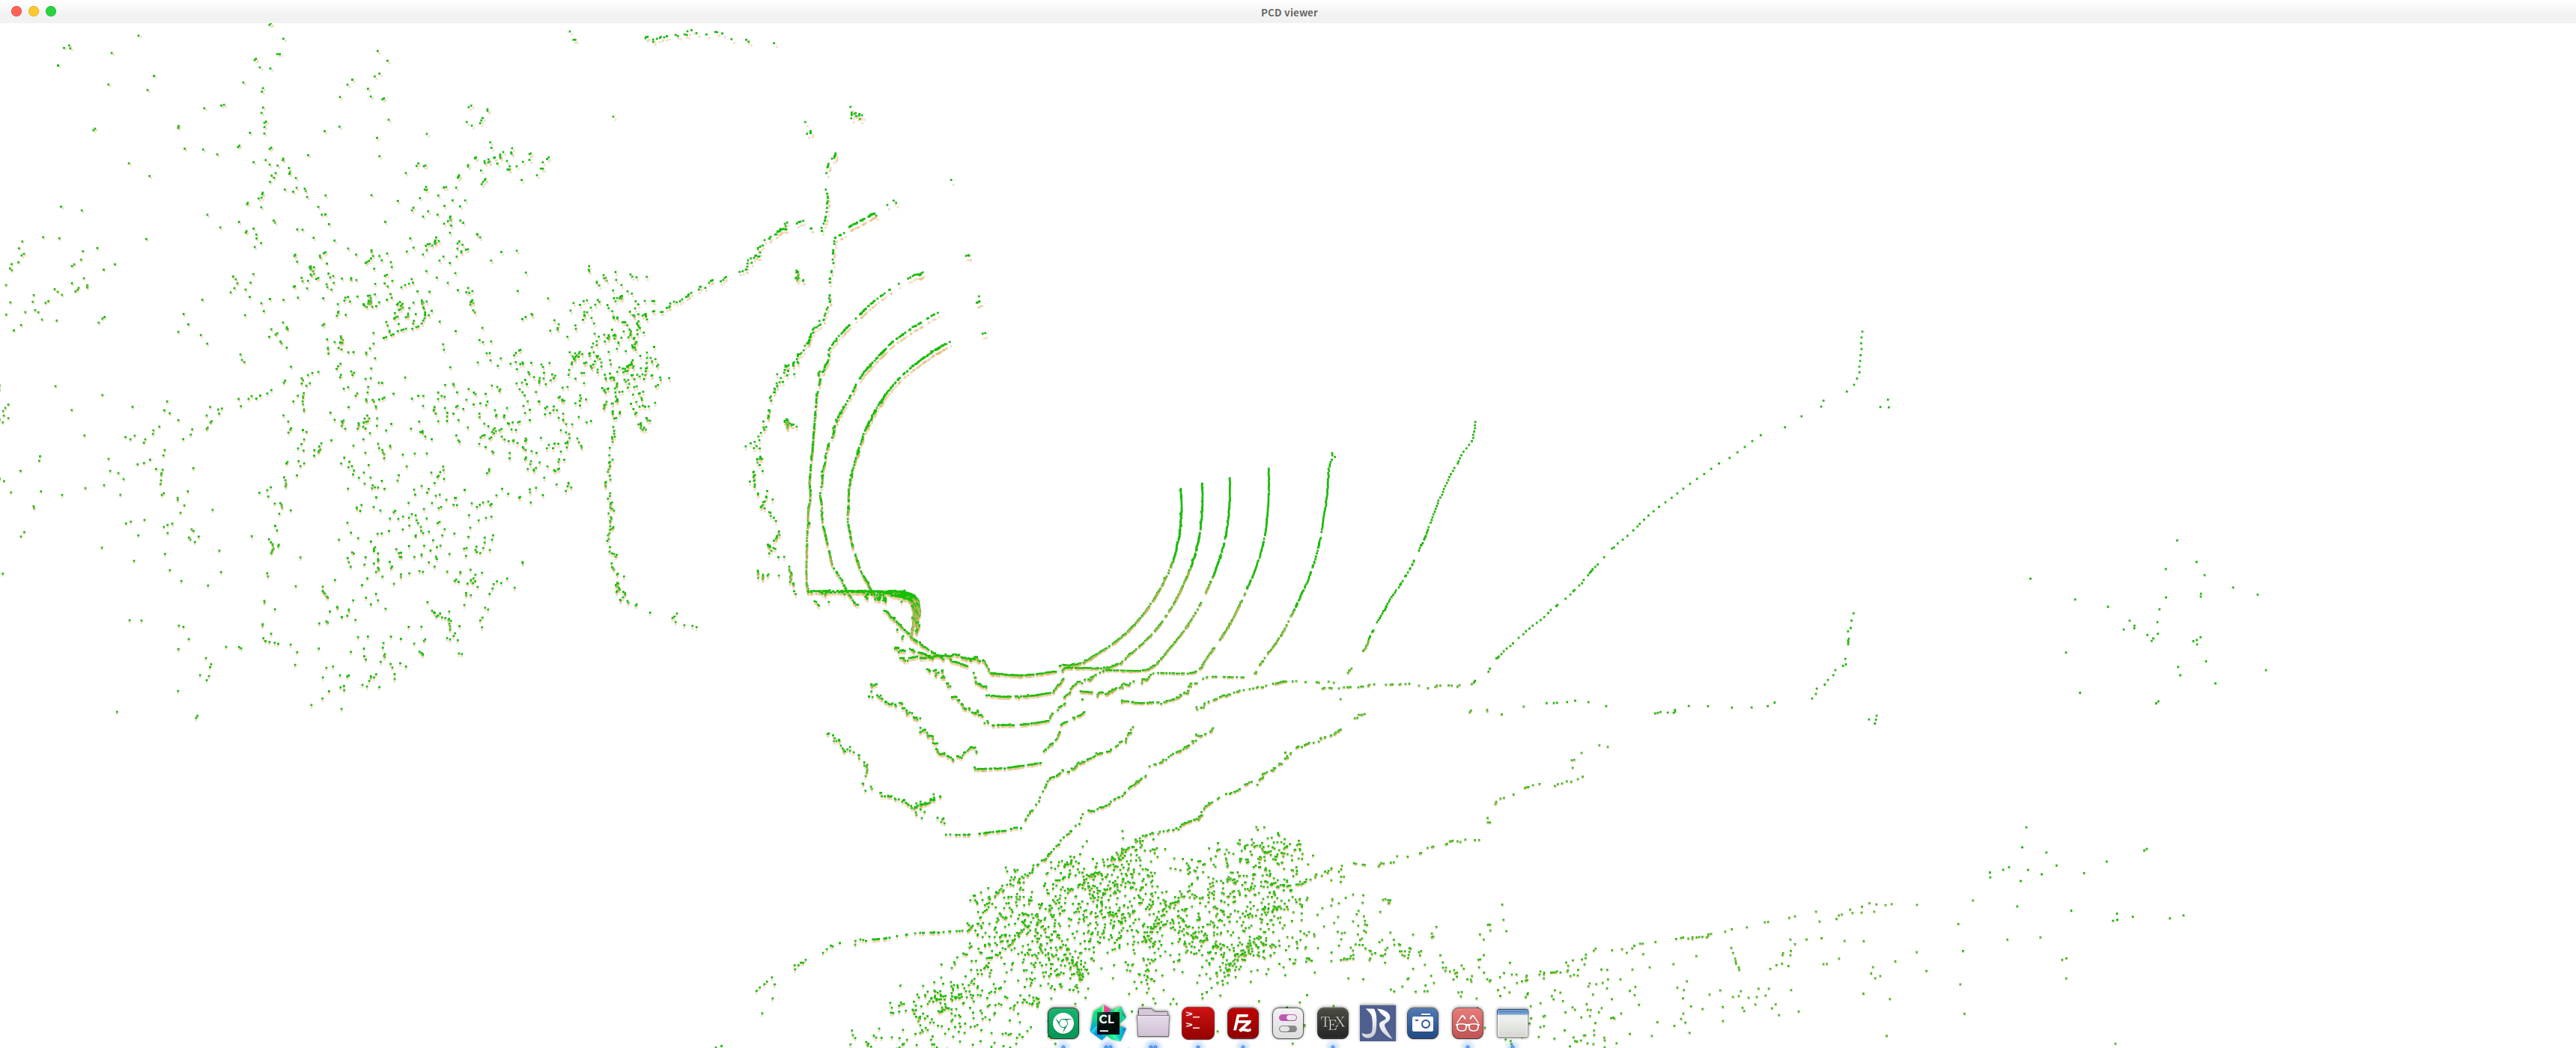
\includegraphics[width=0.8\textwidth]{resources/3d-lidar-mapping/cloud_undist}
	\caption{Point cloud before/after undistortion (green: corrected)}
	\label{fig:cloud-undist}
\end{figure}

\subsection{Registration Module of the Loosely Coupled LIO System}
Finally, we present the registration module code of the loosely coupled LIO system. Since the undistorted point cloud has already been obtained in previous steps, we only need to pass it to the NDT odometry, compute the pose, and then feed it back to the Kalman filter:

\begin{lstlisting}[language=c++,caption=src/ch7/loosely_coupled_lio/loosly_lio.cc]
	void LooselyLIO::Align() {
		FullCloudPtr scan_undistort_trans(new FullPointCloudType);
		pcl::transformPointCloud(*scan_undistort_, *scan_undistort_trans, TIL_.matrix());
		scan_undistort_ = scan_undistort_trans;
		
		auto current_scan = ConvertToCloud<FullPointType>(scan_undistort_);
		
		// Voxel filtering
		pcl::VoxelGrid<PointType> voxel;
		voxel.setLeafSize(0.5, 0.5, 0.5);
		voxel.setInputCloud(current_scan);
		
		CloudPtr current_scan_filter(new PointCloudType);
		voxel.filter(*current_scan_filter);
		
		/// Process first frame of LiDAR data
		if (flg_first_scan_) {
			SE3 pose;
			inc_ndt_lo_->AddCloud(current_scan_filter, pose);
			flg_first_scan_ = false;
			return;
		}
		
		/// Get predicted pose from EKF, feed to LO, obtain LO pose, and finally integrate into EKF
		SE3 pose_predict = eskf_.GetNominalSE3();
		inc_ndt_lo_->AddCloud(current_scan_filter, pose_predict, true);
		pose_of_lo_ = pose_predict;
		eskf_.ObserveSE3(pose_of_lo_, 1e-2, 1e-2);
		
		if (options_.with_ui_) {
			// Send to UI
			ui_->UpdateScan(current_scan, eskf_.GetNominalSE3());  // Convert to Lidar Pose for UI
			ui_->UpdateNavState(eskf_.GetNominalState());
		}
		frame_num_++;
	}
\end{lstlisting}

Now please run the test\_loosely\_lio program to evaluate the performance of this chapter's implementation. The program supports running on three datasets: ULHK, KITTI, and NCLT. You can specify which dataset to use through gflags, for example:
\begin{lstlisting}
	./bin/test_loosely_lio --bag_path ./dataset/sad/nclt/20120429.bag --dataset_type NCLT --config ./config/velodyne_nclt.yaml
\end{lstlisting}

This will run on a specified NCLT data bag. The NCLT data should appear as shown in Figure~\ref{fig:nclt-loosely-lio}. This example program can also run on solid-state LiDAR datasets, such as the AVIA dataset:

\begin{lstlisting}
	bin/test_loosely_lio --bag_path ./dataset/sad/avia/HKU_MB_2020-09-20-13-34-51.bag --config ./config/avia.yaml --dataset_type=AVIA
\end{lstlisting}

The AVIA dataset uses DJI's solid-state LiDAR, where you can observe its field of view is significantly narrower than 360-degree mechanical LiDARs (Figure~\ref{fig:avia-loosely-lio}).

\begin{figure}[!t]
	\centering
	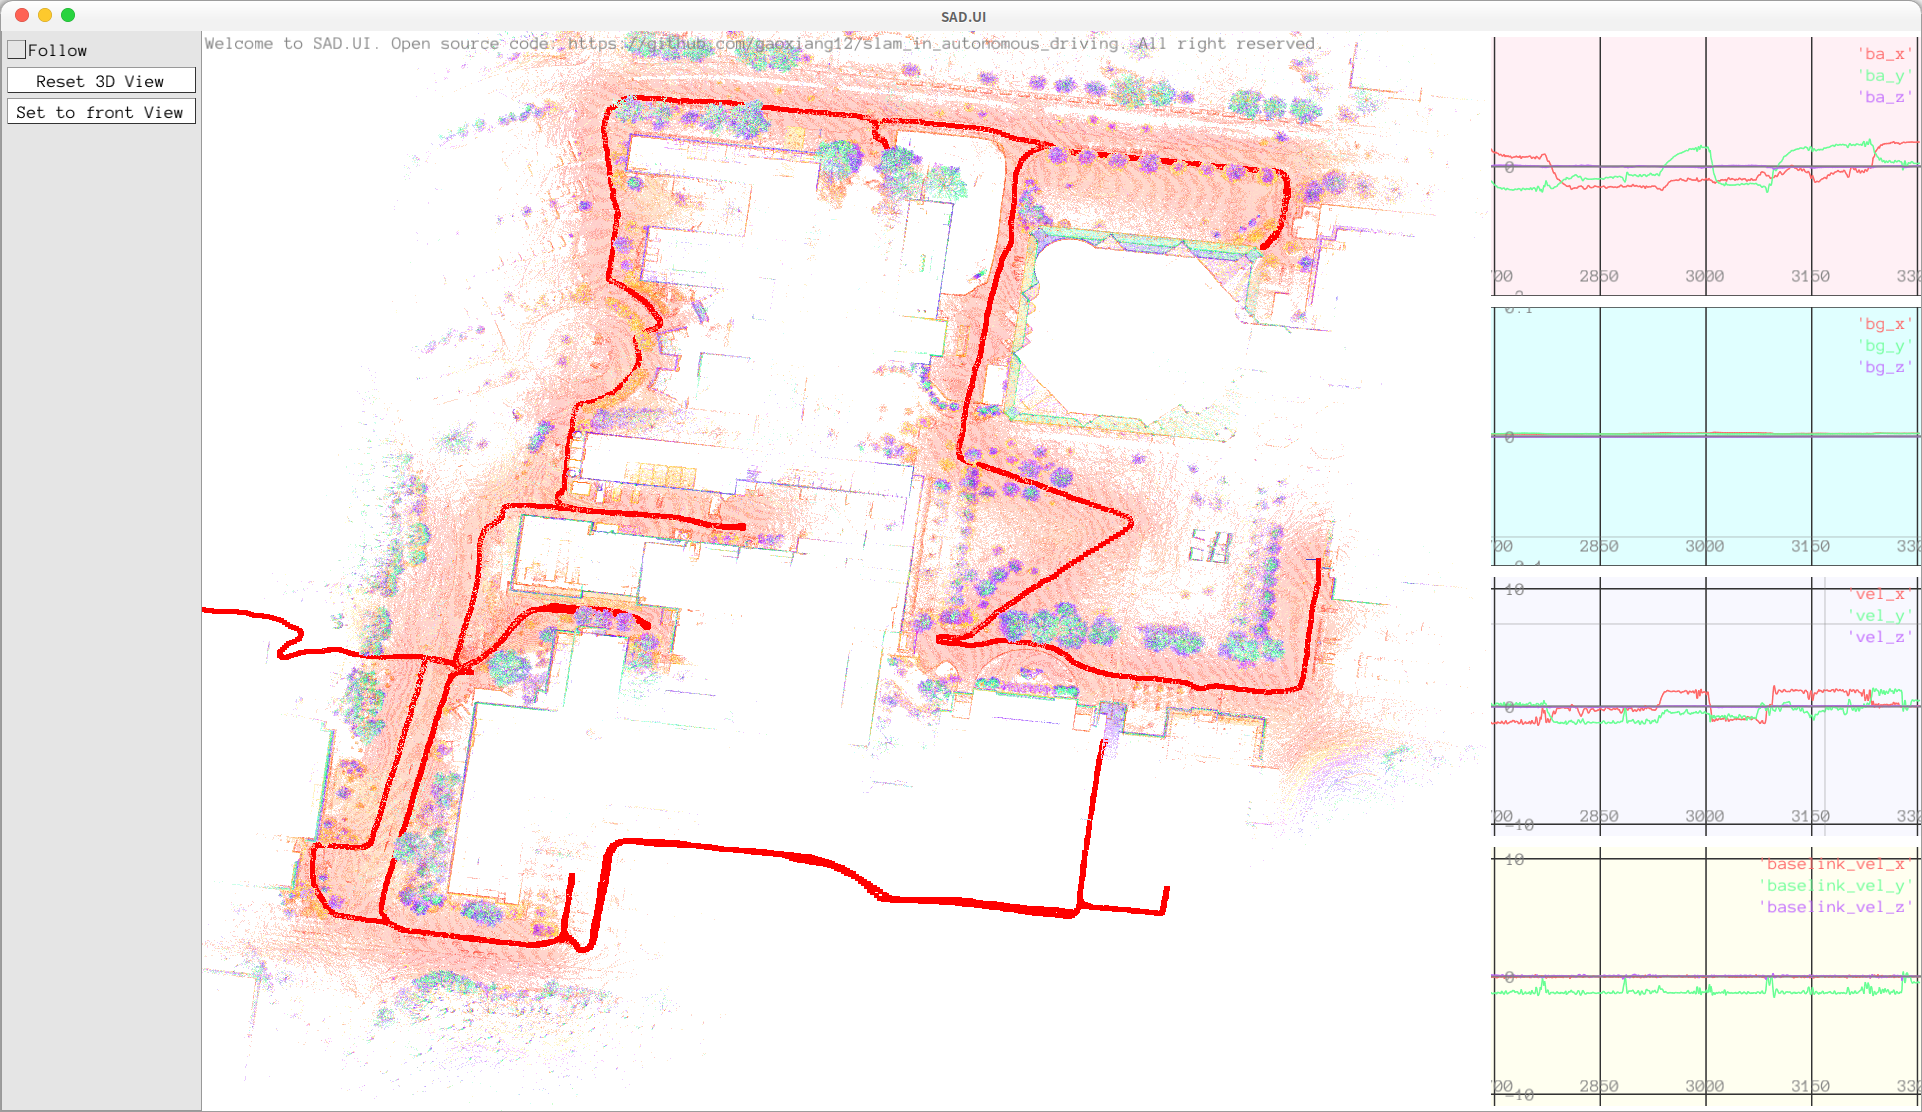
\includegraphics[width=0.8\textwidth]{resources/3d-lidar-mapping/loosely-nclt.png}
	\caption{Real-time operation results of the loosely coupled LIO program on NCLT dataset}
	\label{fig:nclt-loosely-lio}
\end{figure}

\begin{figure}[!t]
	\centering
	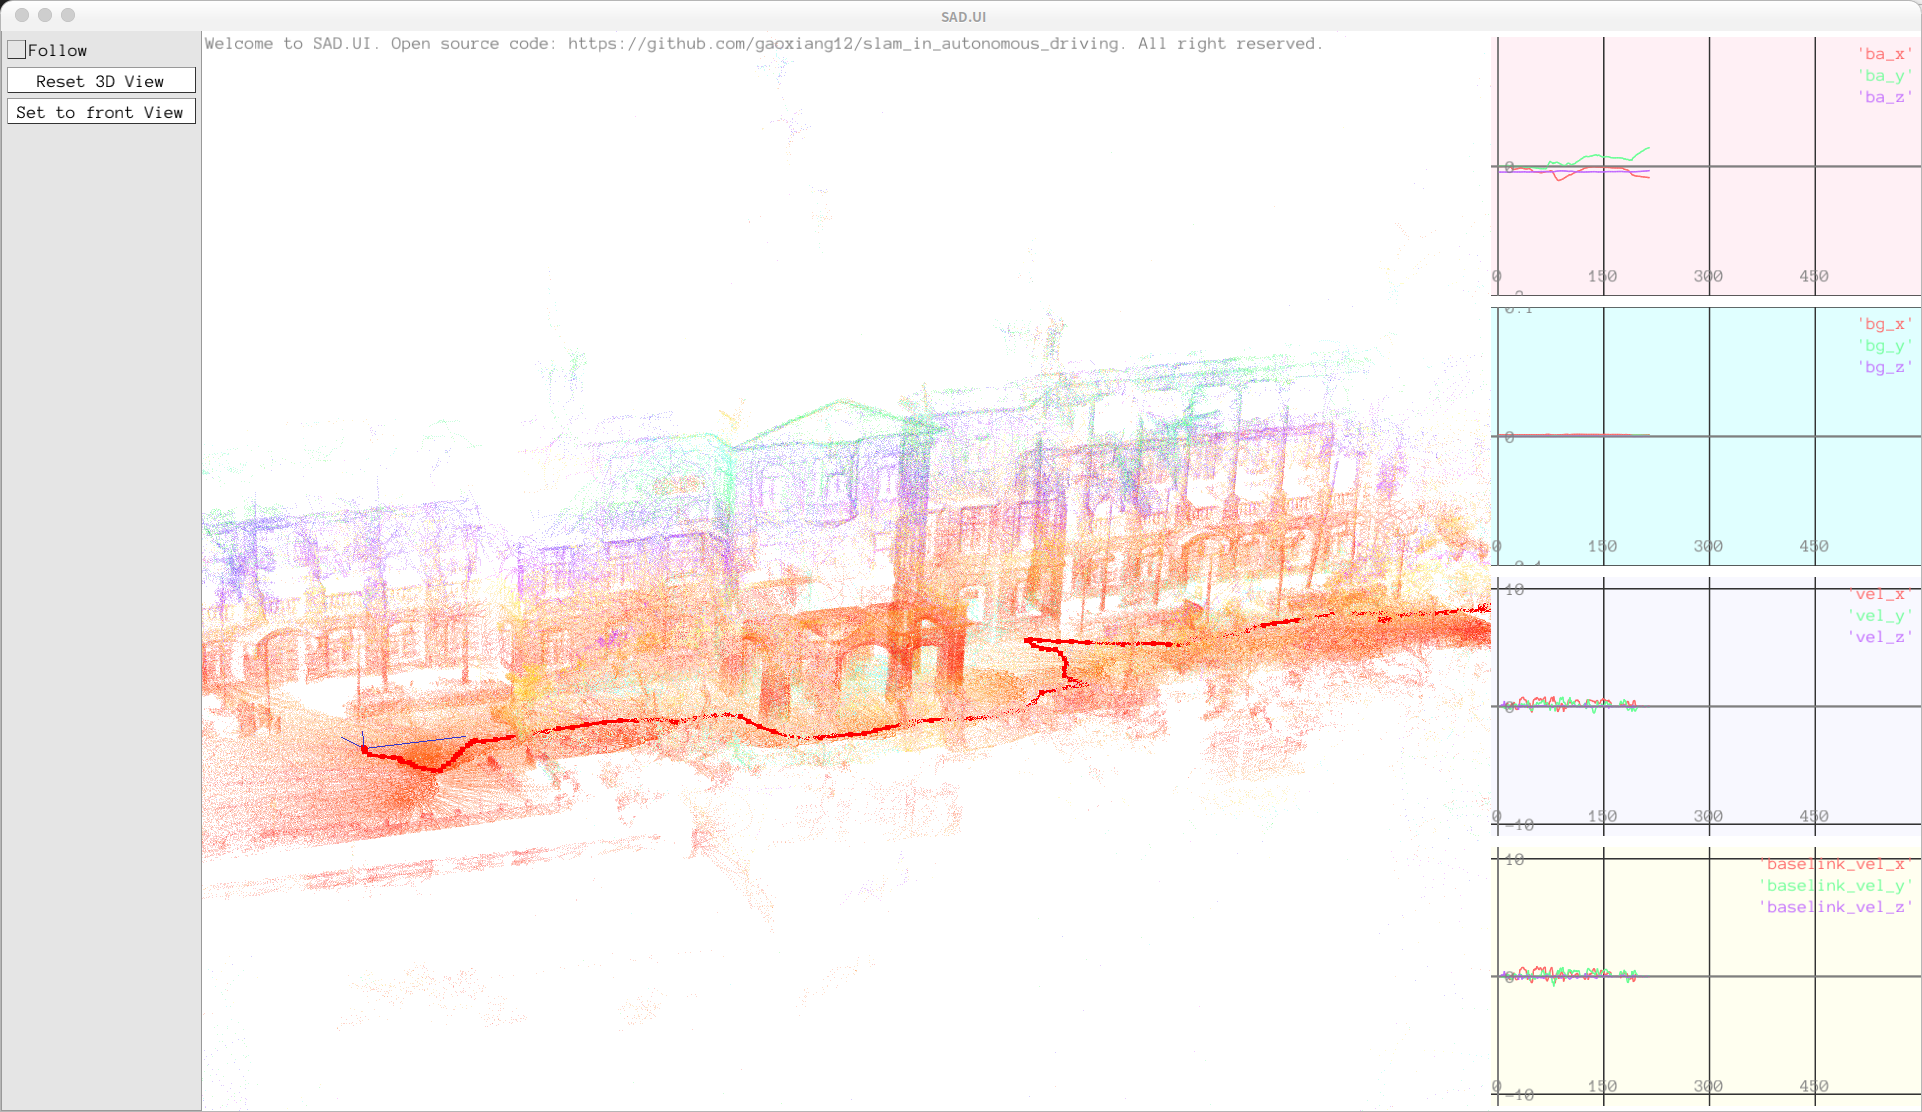
\includegraphics[width=0.8\textwidth]{resources/3d-lidar-mapping/avia01.png}
	\caption{Real-time operation results of the loosely coupled LIO program on AVIA dataset}
	\label{fig:avia-loosely-lio}
\end{figure}


\section{Summary}
This section systematically introduced the fundamental algorithms of a 3D LiDAR SLAM system. We implemented various ICP and NDT methods and extended them into LiDAR odometry. Furthermore, we realized feature-based LiDAR odometry and, combined with the previous Kalman filter, implemented a loosely coupled LIO system based on the Kalman filter. Through the programs in this section, readers can gain deeper insight into how a point cloud system is composed and operates.

In the next section, we will focus on tightly coupled LIO systems. We will introduce tightly coupled LIO based on iterative Kalman filters and optimization. Subsequently, we will incorporate RTK constraints and loop closure detection constraints to achieve complete mapping and localization functionality.

\section*{Exercises}
\begin{enumerate}
	\item Derive the right multiplication derivative of $\mathbf{R}$ in Equation \eqref{eq:p2p-icp-jacobian}.
	\item Use std::reduce to parallelize the Hessian matrix accumulation process.
	\item Derive the derivatives of point-to-plane and point-to-line residuals with respect to $\mathbf{R}$.
	\item Explain the relationship between weighted least squares problems and maximum likelihood estimation in NDT.
	\item Design and implement a parallel computation pipeline for calculating laser beam curvature.
	\item Develop a ground extraction pipeline for the LOAM-like odometry in this book, and apply point-to-plane ICP separately to ground point clouds.
	\item Study relevant literature to understand the differences in feature extraction methods between algorithms like LOAM or LeGO-LOAM.
	\item *Attempt to implement a loosely coupled LIO system using other methods introduced in this book (point-to-plane ICP, feature-based methods, etc.).
\end{enumerate}

